
\documentclass[draftthesis,tocnosub,noragright,centerchapter,12pt]{uiucthesis17}

% Use draftthesis for notes and date markings on every page.  Useful when you
%   have multiple copies floating around.
% Use offcenter for the extra .5 inch on the left side. Needed with fullpage and fancy.
% Use mixcasechap for compatibility with hyperref package, which does NOT like all caps default
% Use edeposit for the adviser/committee on the title page.
% Use tocnosub to suppress subsection and lower entries in the TOC.
% PhD candidates use "proquest" for the proquest abstract.

%%%%%%%%%%%%%%%%%%%%%%%%%%%%%%%%%%%%%%%%%%
% Packages
%%%%%%%%%%%%%%%%%%%%%%%%%%%%%%%%%%%%%%%%%%
\makeatletter
\usepackage{graphicx}		% For \includegraphics
\graphicspath{{figures/}}	% Looks under ../Data/figures/ sub-dir for files referenced by \includegraphics
\usepackage{setspace}
\usepackage{epsfig}  % for figures
%\usepackage{graphicx}  % another package that works for figures
%\usepackage{subfigure}  % for subfigures
\usepackage{amsmath}  % for math spacing
%\usepackage{amssymb}  % for math spacing
%\usepackage{url}  % Hyphenation of URLs.
\usepackage{lscape}  % Useful for wide tables or figures.
\usepackage[justification=raggedright]{caption}	% makes captions ragged right - thanks to Bryce Lobdell
\usepackage{amsmath}		% For \begin{bmatrix}
\usepackage{color}			% For \textcolor
\usepackage{verbatim}



%%%%%%%%%%%%%%%%%%%%%%%%%%%%%%%%%%%%%%%%%%
% Commands
%%%%%%%%%%%%%%%%%%%%%%%%%%%%%%%%%%%%%%%%%%
\newcommand{\Bezier}{B\'ezier}
\renewcommand{\(}{\left(}
\renewcommand{\)}{\right)}
\newcommand{\dq}{{\dot{q}}}
\newcommand{\ddq}{{\ddot{q}}}
\newcommand{\dz}{{\dot{z}}}
\newcommand{\ddz}{{\ddot{z}}}
\newcommand{\dJ}{{\dot{J}}}
\newcommand{\dJx}{{\dot{J_x}}}

% Uncomment the appropriate one of the following four lines:
\msthesis
%\phdthesis
%\otherdoctorate[abbrev]{Title of Degree}
%\othermasters[abbrev]{Title of Degree}


%%%%%%%%%%%%%%%%%%%%%%%%%%%%%%%%%%%%%%%%%%
% Title
%%%%%%%%%%%%%%%%%%%%%%%%%%%%%%%%%%%%%%%%%%
\title{Design and Experimental Implementation of a Quasi-Direct-Drive Leg for Optimized Jumping}
\author{Yanran Ding}
\department{Mechanical Science and Engineering}
\degreeyear{2017}

% Advisor name is required for
% - doctoral students for the ProQuest abstract
% - master's students who do not have a master's committee
\advisor{Hae-Won Park}

% Uncomment the \committee command for
% - all doctoral students
% - master's students who have a master's committee
%\committee{Professor Firstname Lastname, Chair\\
%        Professor Firstname Lastname} % etc.

\begin{document}

%%%%%%%%%%%%%%%%%%%%%%%%%%%%%%%%%%%%%%%%%%%%%%%%%%%%%%%%%%%%%%%%%%%%%%%%%%%%%%%
% COPYRIGHT
%
%\copyrightpage
%\blankpage

%%%%%%%%%%%%%%%%%%%%%%%%%%%%%%%%%%%%%%%%%%%%%%%%%%%%%%%%%%%%%%%%%%%%%%%%%%%%%%%
% TITLE
%
\maketitle

%\raggedright
\parindent 1em%

\frontmatter

%%%%%%%%%%%%%%%%%%%%%%%%%%%%%%%%%%%%%%%%%%%%%%%%%%%%%%%%%%%%%%%%%%%%%%%%%%%%%%%
% ABSTRACT
%
\begin{abstract}
% Put the abstract in a file called "abs.tex" and it'll be inputted here.
Input your text here
\end{abstract}


%%%%%%%%%%%%%%%%%%%%%%%%%%%%%%%%%%%%%%%%%%%%%%%%%%%%%%%%%%%%%%%%%%%%%%%%%%%%%%%
% DEDICATION
%
\begin{dedication}
% Whatever dedication you want.
To my parents, for their love and support.
\end{dedication}

%%%%%%%%%%%%%%%%%%%%%%%%%%%%%%%%%%%%%%%%%%%%%%%%%%%%%%%%%%%%%%%%%%%%%%%%%%%%%%%
% ACKNOWLEDGMENTS
%
% Put acknowledgments in a file called "ack.tex" and it'll be inputted here.
\begin{acknowledgments}
Input your text here
\end{acknowledgments}

%%%%%%%%%%%%%%%%%%%%%%%%%%%%%%%%%%%%%%%%%%%%%%%%%%%%%%%%%%%%%%%%%%%%%%%%%%%%%%%
% TABLE OF CONTENTS
%
\tableofcontents

%%%%%%%%%%%%%%%%%%%%%%%%%%%%%%%%%%%%%%%%%%%%%%%%%%%%%%%%%%%%%%%%%%%%%%%%%%%%%%%
% LIST OF TABLES
%
% The List of Tables is not strictly necessary. Omitting the List of Tables will
% simplify the thesis check and reduce the number of corrections.
\listoftables

%%%%%%%%%%%%%%%%%%%%%%%%%%%%%%%%%%%%%%%%%%%%%%%%%%%%%%%%%%%%%%%%%%%%%%%%%%%%%%%
% LIST OF FIGURES
%
% The List of Figures is not strictly necessary. Omitting the List of Figures will
% simplify the thesis check and reduce the number of corrections.
\listoffigures

%%%%%%%%%%%%%%%%%%%%%%%%%%%%%%%%%%%%%%%%%%%%%%%%%%%%%%%%%%%%%%%%%%%%%%%%%%%%%%%
% LIST OF ABBREVIATIONS
%
% The List of Abbreviations is not strictly necessary.
\chapter{LIST OF ABBREVIATIONS}

%\begin{symbollist*}
%\item[EPIC] Explicitly Parallel Instruction Computing
%\item[GPU] Graphics Processing Unit
%\item[VLIW] Very Long Instruction Word
%\end{symbollist*}


%%%%%%%%%%%%%%%%%%%%%%%%%%%%%%%%%%%%%%%%%%%%%%%%%%%%%%%%%%%%%%%%%%%%%%%%%%%%%%%
% LIST OF SYMBOLS
%
%\begin{symbollist}[0.7in]
%\item[$\tau$] Time taken to drink one cup of coffee.
%\end{symbollist}

\mainmatter

%%%%%%%%%%%%%%%%%%%%%%%%%%%%%%%%%%%%%%%%%%%%%%%%%%%%%%%%%%%%%%%%%%%%%%%%%%%%%%%
% INSERT REAL CONTENT HERE
%

\chapter{Introduction}
This is my introduction.
\section{Motivation}

\section{State of Art}

\section{Contribution}

\section{Thesis Outline}


	% for INTRODUCTION in "intro.tex"

\chapter{System Modeling}
\section{System Modeling}
\label{sec:systemModel}

A sequential and iterative design process was adopted to refine simulation model and mechanical design as shown in Figure \ref{fig:systemOverview}. The 1-DOF template \cite{Full1999} called \textbf{knee extensor model} was used to investigate the torque and angular speed requirement of the leg, as depicted in Figure \ref{fig:systemOverview}(a). It assumes all masses are lumped at the base; thigh and shank link are of same length and have no mass or inertia; foot is located directly below the hip, which means no horizontal off-set for foot hold. Jumping motion was simulated using this knee extensor model under various motors' maximal speed and maximal torque. These simulations in turn exposed the speed and torque requirements in order to achieve the desired motion, which provides guidance for choosing appropriate motor and gear ratio.

A more detailed leg model with motors' rotary inertia and horizontal foot off-set was introduced as shown in Figure \ref{fig:systemOverview} (b). The detailed leg model was used to further narrow the choice of gear ratio by minimizing ground impact force while maintaining balance between torque and speed requirements. Optimized parameters were tested on the hardware platform shown in Figure \ref{fig:systemOverview} (c) to validate the design.

\begin{figure}
	\centering
	\resizebox{1.0\linewidth}{!}{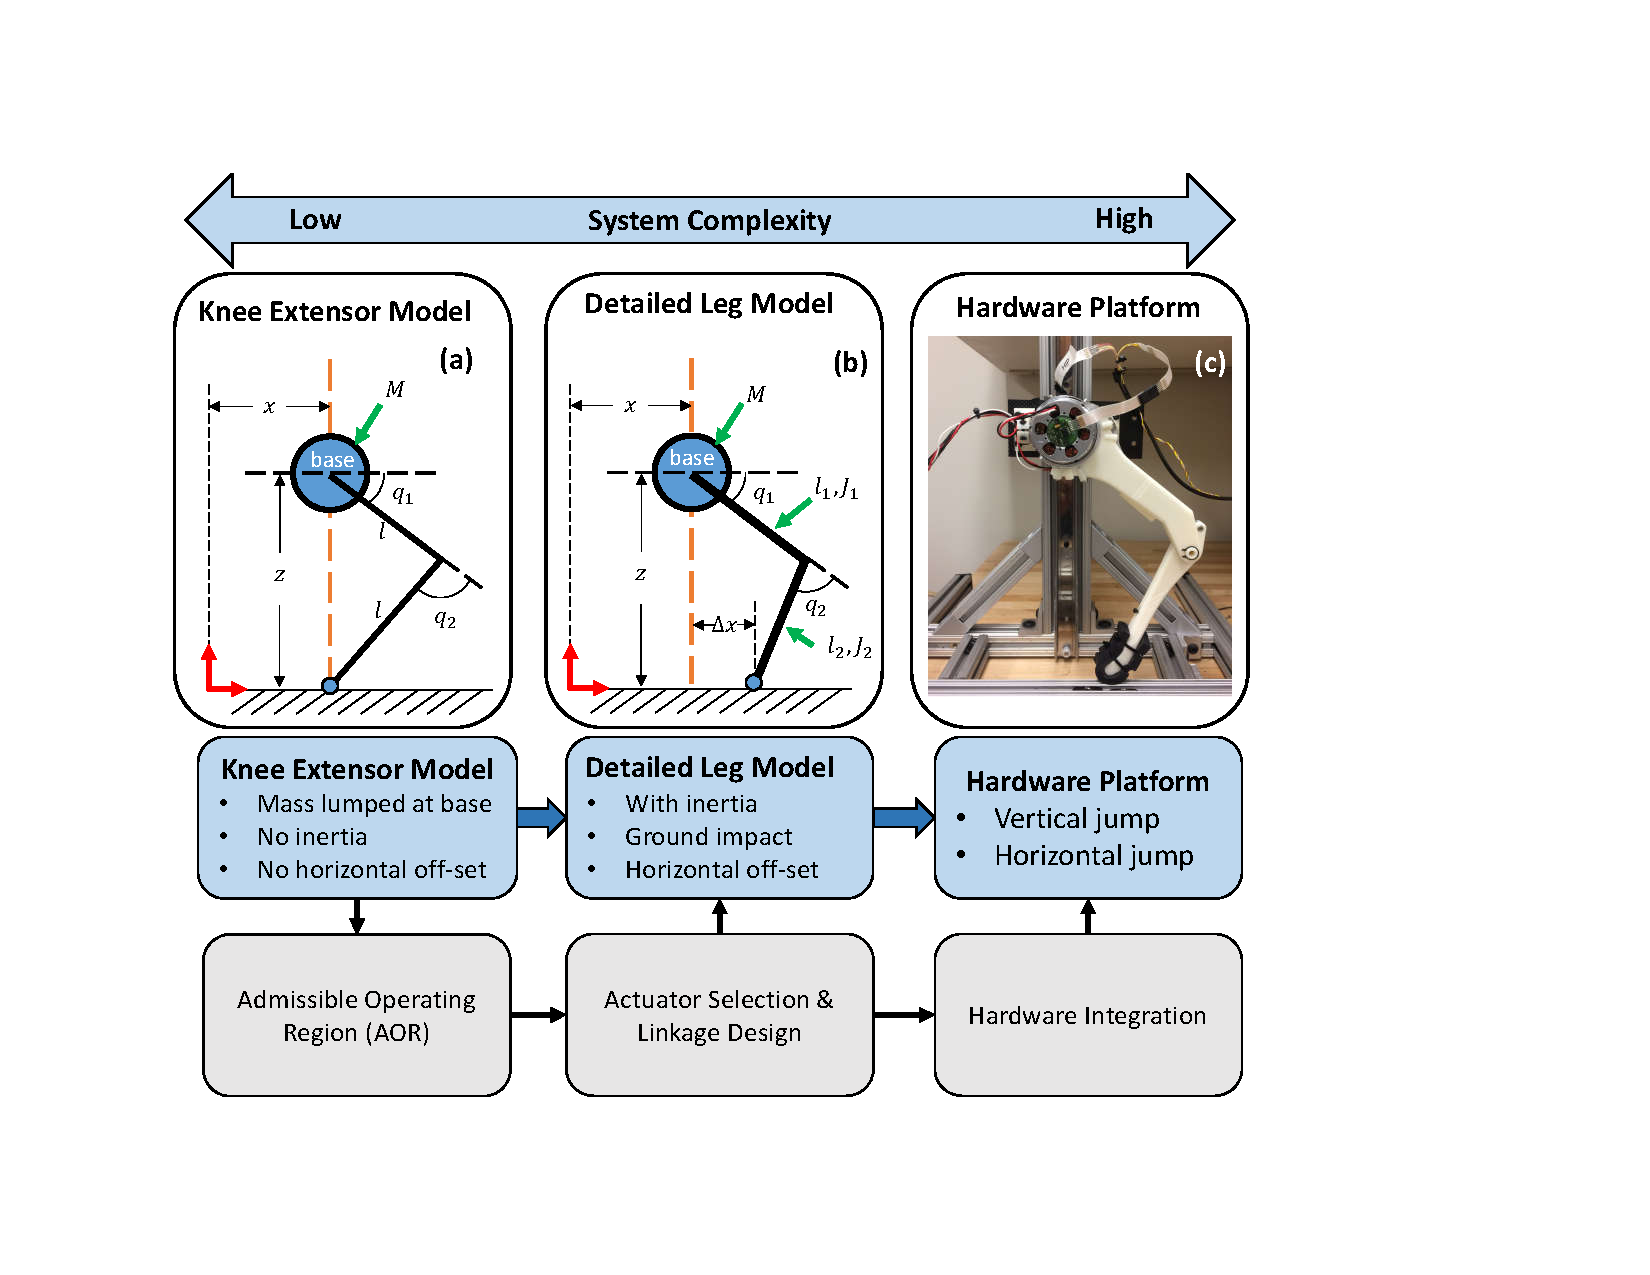
\includegraphics{system_overview.pdf}}
	\caption{Sequential design process for determining design parameters. (a) knee extensor model for motor selection (b) detailed leg model for linkage design and gear ratio choice (c) hardware platform for experiments}
	\label{fig:systemOverview}
\end{figure}

%-------------------------------------------
% ----------Knee Extensor Model----------
\subsection{Knee Extensor Model}
\label{sec:kneeExtensorModel}

The knee extensor model was used to estimate the torque and speed requirements to achieve desirable jumping motions, which provides us with an initial guidance for choosing motor and gearbox. Figure \ref{fig:systemOverview} (a) shows the schematics of the knee extensor model. The model assumes that all masses are lumped at the base to be $M$, which is mounted on a vertical linear rail. Thigh and shank links have an identical length of $l$, while its foot and base are vertically aligned. Hence only the knee joint needs to be actuated to perform vertical jump while the hip joint is not actuated. The vertical height of the base $z$ and joint angles $q_1, q_2$ are shown in Figure \ref{fig:systemOverview}.

The dynamics of this model was formalized as a single point mass accelerated due to ground reaction force (GRF). Ground reaction force was chosen as the control input because it is the only external force in the knee extensor model that could increase the mechanical energy of the system. The equation of motion (EOM) of the system is: $\ddz = \frac{F_z}{M}-g$, where $z$ is the vertical displacement of the base, $F_z$ is the vertical component of GRF, $M$ is the lumped mass at the base and $g$ is the gravitational acceleration. 

%-------------------------------------------
% ----------GRF Parameterized as \Bezier\ Polynomial----------
\subsection{GRF Parameterized as \Bezier\ Polynomial}
\label{sec:BezierPoly}
	
A $5^{th}$ order \Bezier\ polynomial was used to parameterize the GRF profile. The reasons for using \Bezier\ Polynomial to parametrize the ground reaction force is two fold. Firstly, the first and last coefficient of a \Bezier\ polynomial corresponds to the initial and final value of the GRF, which makes it more convenient to anchor GRF to desired values at the initial and final instance; secondly, integration of \Bezier\ Polynomial is a linear operation, which is computationally inexpensive. This property is utilized in integrating the prescribed ground reaction force and integrate to get the velocity trajectory, as shown in Equation \ref{eq:bernstein_integration}, and integrate again to get the position trajectory

The coefficients of \Bezier\ polynomial are assumed to be $[Mg, \alpha_1, \alpha_2, \alpha_3, \alpha_4, 0]$. The first coefficient was set to be the weight of the leg because it is assumed that the leg starts from static equilibrium state, and last coefficient was set as $0$ to ensure a smooth and physically feasible motion at the take-off moment.  

The Bernstein polynomials are defined over [0,1] as:

\begin{equation}
	B_{i,N} = \left(
	\begin{smallmatrix}
	N\\
	i
	\end{smallmatrix}\right)
	x^i(1-x)^{n-i},
	0\leq i \leq N
\end{equation}
where  $\left(
\begin{smallmatrix}
N\\
i
\end{smallmatrix}\right)$
is the binomial coefficients.

Since a \Bezier\ polynomial is the linear combination of a Bernstein polynomial basis\cite{dicsibuyuk2007generalization} defined as,

\begin{equation}\label{eq:bezier}
C_N(s) = \sum_{i=0}^{N}\alpha_i B_{i,N}(s)
\end{equation}

where $\alpha_i$ is the coefficient for the $i^{th}$ Bernstein polynomial $B_{i,N}$, analytical solution for velocity and position could be obtained using the property of the Bernstein polynomial\cite{Doha2011}:

\begin{equation} \label{eq:bernstein_diff}
\frac{d}{ds}B_{i,N}(s)=\frac{N}{T}(B_{i-1,N-1}(s)-B_{i,N-1}(s))
\end{equation}
where $s$ is a point between general time interval $[0, T]$.

Given the initial velocity $\dz_0$, the velocity trajectory in stance phase is a $6^{th}$ order \Bezier\ polynomial with coefficients $\gamma_{(0-6)}$. The linear relationship between force and velocity \Bezier\ coefficient is:

\begin{equation}\label{eq:bernstein_integration}
\frac{6}{T_{st}}\left[
\begin{smallmatrix}
-1 & 1 & 0 & 0 & 0 & 0 & 0 \\
0 &-1 & 1 & 0 & 0 & 0 & 0 \\
0 & 0 &-1 & 1 & 0 & 0 & 0 \\
0 & 0 & 0 &-1 & 1 & 0 & 0 \\
0 & 0 & 0 & 0 &-1 & 1 & 0 \\
0 & 0 & 0 & 0 & 0 &-1 & 1 \\
1 & 0 & 0 & 0 & 0 & 0 & 0 \\
\end{smallmatrix}
\right]
\left[
\begin{matrix}
\gamma_0\\\gamma_1\\\gamma_2\\\gamma_3\\\gamma_4\\\gamma_5\\\gamma_6\\
\end{matrix}
\right]
=
\left[
\begin{matrix}
\left[
\begin{matrix}
0\\\alpha_1\\\alpha_2\\\alpha_3\\\alpha_4\\0\\
\end{matrix}
\right]\frac{1}{M}-g\\
\dz_0\\
\end{matrix}
\right]
\end{equation}
where $T_{st}$ is the stance duration for jumping up.

Similarly, the position trajectory in stance phase could also be integrated by applying the linear operation shown in Equation \ref{eq:bernstein_integration} given initial position $z_0$. At each instance  $t\in[0,T_{st} ]$, the joint angle $q=[q_1,q_2]$ defined in Figure \ref{fig:systemOverview}(a) was solved by inverse kinematics. 

Since the thigh and shank links are assumed to be massless, joint torque $\tau=[\tau_1,\tau_2]$ could be reconstructed using 
\begin{equation}
	\tau=J(q)^T F
\end{equation}

where $\tau_1$ and $\tau_2$ are joint torques for hip and knee joints, $F$ is the ground reaction force, and $J(q)\in R^{2\times 2} $ is the manipulator Jacobian of the foot relative to the hip.

The jumping performance was evaluated by the maximal reachable height $h_{max}$,
 \begin{equation}
 	 h_{max} := h_{to}+\frac{v_{to}^2}{2g}
 \end{equation}

 where $h_{to}$ and $v_{to}$ are the base height and speed at the moment of take-off.

%---------------------------------------------------------------------
% ----------Nonlinear Optimization for Ground Reaction Force----------
\subsection{Nonlinear Optimization for Ground Reaction Force}
\label{sec:nonlOptGRF}

In order to get the optimal ground reaction force profile within actuator limits, an optimal control problem was formulated and solved using nonlinear optimization:
\begin{equation}\label{eq:path_constraints}
\begin{aligned}
\min&~~~~~~~~~~-h_{max}\\
s.t.&~~~~~~~q_{lb}\leq q \leq q_{ub}\\
&~~~~~~~\dq_{lb}\leq \dq \leq \dq_{ub}\\
&~~~~~~~\tau_{lb}\leq \tau \leq \tau_{ub}\\			 	
\end{aligned}
\end{equation}
where $q_{lb}$, $q_{ub}$ are the lower and upper bounds for joint angles; $\dq_{lb}$, $\dq_{ub}$ for angular velocity; $\tau_{lb}$, $\tau_{ub}$ for joint torques.  

Dynamics was discretized at $N$ sampling points to search for optimal variable values. Joint angle $q$ and angular velocity $\dq$ were discretized at the sampling points. Motor's maximal speed and torque constraints were imposed at each sampling point as inequality constraints.

The optimization variables are chosen as follows:
\begin{equation}\label{eq:opt_var_knee}
x_{opt} = [z_0, \alpha_{(1-4)}, T_{st}, q_{(1-N)}, \dq_{(1-N)}]
\end{equation}
where $x_{opt}$ is the vector of optimization variables for stance phase; $z_0$ is the base's vertical initial position; $\alpha_{(1-4)}$ are the \Bezier\ polynomial coefficients of ground reaction force; $T_{st}$ is the total stance time; $q$ is the vector of joint angles and $\dq$ is the vector of joint velocities at all the sampling points.

Equality constraints were imposed to satisfy forward kinematics:

\begin{equation}
\label{eq:kin_position}
rot(q_1)
\left[\begin{matrix}
l\\0
\end{matrix}\right]
+
rot(q_1+q_2)\left[\begin{matrix}
l\\0
\end{matrix}\right]
+
\left[\begin{matrix}
0\\z
\end{matrix}\right]
=0
\end{equation}

\begin{equation}
\label{eq:kin_velocity}
J(q)\dq+\left[\begin{matrix}
0\\ \dz
\end{matrix}
\right]
=
\left[\begin{matrix}
0\\0
\end{matrix}\right]
\end{equation}
where $rot\in SO(2)$ is the rotation matrix. $z$ and $\dz$ are the vectors of height and velocity of the base at each sampling point using Equation \ref{eq:bernstein_integration}.


MATLAB's $fmincon$ function was used to search for local optimal solutions. The parameters for the knee extensor model is chosen as follows: mass $M = 0.66~kg$, link length $l=0.12~m$. 100 simulation runs were executed over 10 different maximal motor speed ($\omega_{max}$ from 23 rad/s to 37 rad/s) and maximal torque ($\tau_max$ from 6.2 Nm to 9.7 Nm) constraints, then the maximal achievable height $h_{max}$ is plotted as the third axis against $\tau_{max}$ and $\omega_{max}$. As shown in Figure \ref{fig:hmax_pcolor}, the maximal achievable height increases as the upper limit for speed and torque increases. The level curves shows that $h_{max}$ could reach as high as 0.8 m theoretically with the effective actuator torque of 9.7 Nm and actuator speed of 37 rad/s.

The advantage of this method is that it decoupled the study of jumping to two decoupled problems. In terms of dynamics, it treats the leg as a point mass accelerated due to ground reaction force and gravity; in terms of kinematics, it assumes two link kinematics chain for leg topology. After imposing equality constraints which bridges the error between kinematics as shown in Equations \ref{eq:kin_position} and Equation \ref{eq:kin_velocity}, the problem is tackled in a way that avoids the problem of singularity in the search of optimization variables.


%-----------------------------------------------
% ----------Admissble Operating Region----------
\subsection{Admissble Operating Region}
\label{sec:AOR}

\begin{figure}
	\centering
	\resizebox{1.0\linewidth}{!}{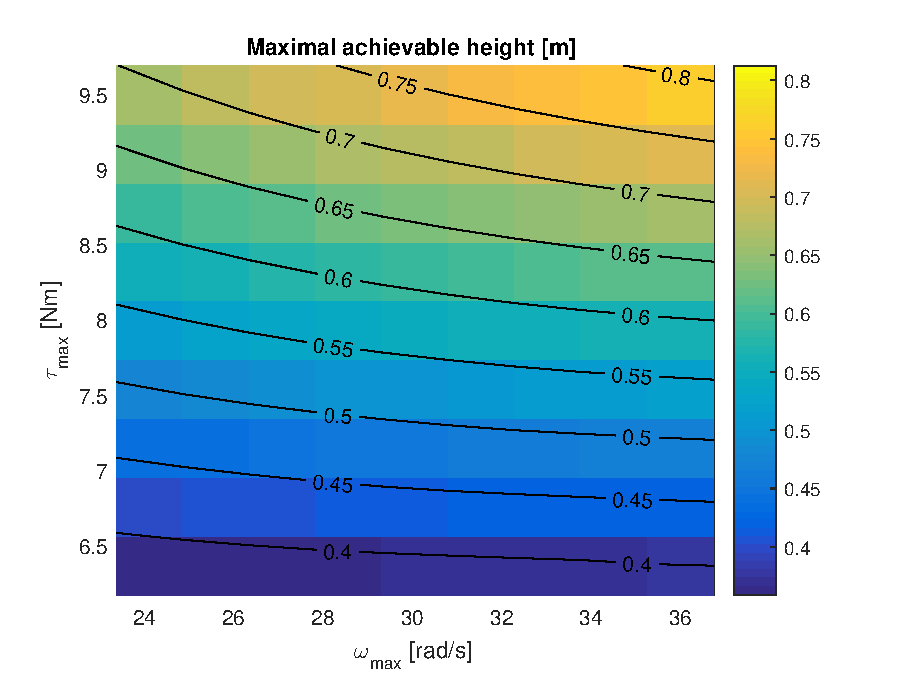
\includegraphics{hmax_pcolor.eps}}
	\caption{Maximal achievable height for specific torque and speed limit. The x-axis corresponds to maximal angular velocity of the actuator, the y-axis corresponds to maximal torque of the actuator, and the depth represents the maximal achievable height of a jump}
	\label{fig:hmax_pcolor}
\end{figure}

\begin{figure}
	\centering
	\resizebox{0.8\linewidth}{!}{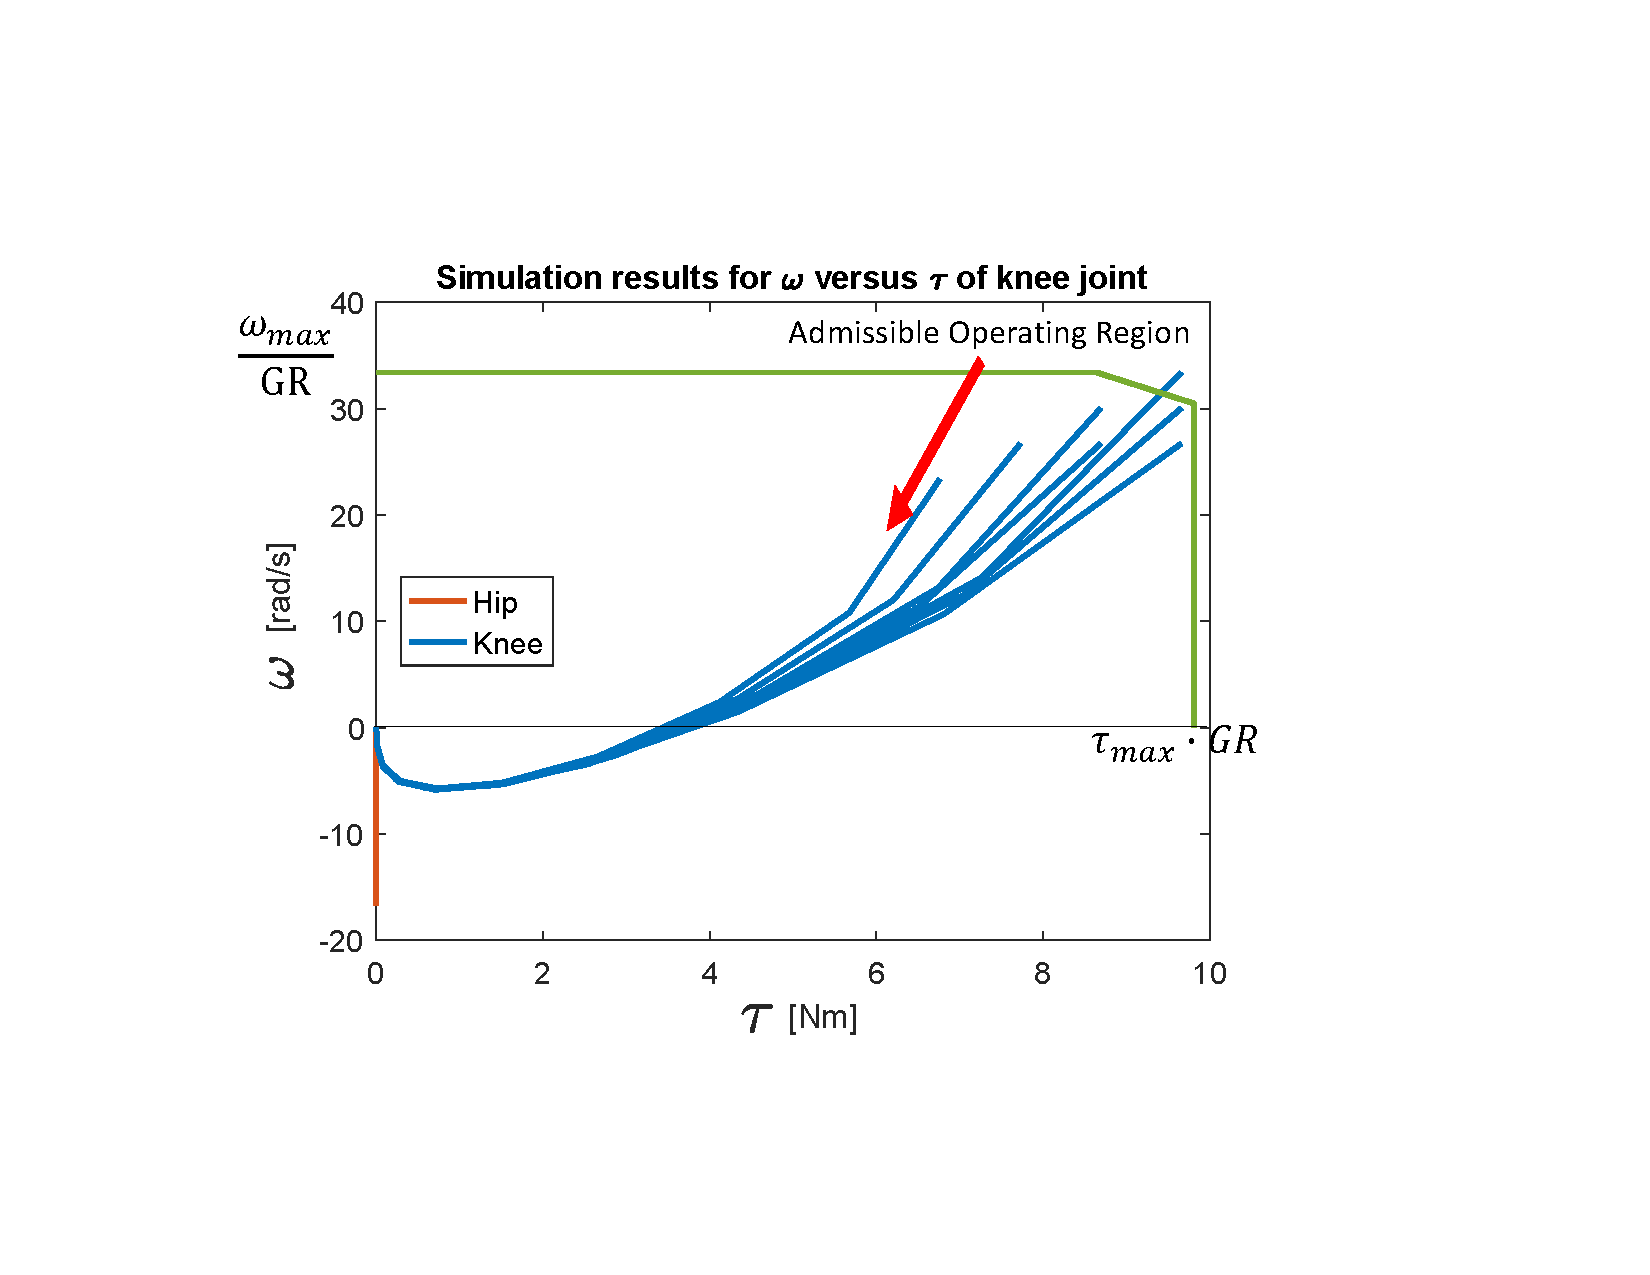
\includegraphics{AOR.pdf}}
	\caption{The Admissible Operating Region (AOR) formed by the torque and angular speed trajectories from the one hundred knee extensor model simulations. A typical motor's speed-torque curve scaled by gear ratio of 23:1 is plotted in green curve. Hip motor acts as a passive joint throughout the jumping up phase.}
	\label{fig:AOR}
\end{figure}

 In general, Admissible Operating Region (AOR) is defined as the area in the torque-speed plane enclosed by the Leg's torque-speed trajectory in performing certain task, as is shown in Figure \ref{fig:AOR}. The motions corresponding to the enclosed AOR region are admissible to the actuator. It is a projection of dynamic motion to the torque-speed domain of the actuators. It is a lumped quantity which treats the motor and gearbox as a unity instead of separating the characteristics of both. The contribution of the proposition of AOR is that it captures the essence of robot motion generation, and bridges between motor dynamics, and workspace dynamics. Furthermore, it could be used in the early stage of design by projecting workspace dynamics to actuator's speed-torque space, before the choice of motor and transmission design is determined. 
 
 \subsubsection{Scaling Effect of Gear Ratio}
 \label{sec:GR_scale_effect}
 
 The analysis of AOR takes motor and gearbox as a whole entity. Since AOR is determined by desired motion, it does not change with gear ratio, hence it is independent of actuator and gearbox choices. What the gear ratio could scale is the motor characteristic curve. Shown as the green curve in Figure \ref{fig:AOR}, the original speed-torque curve of this specific motor is scaled by gear ratio to enclose more of the AOR. Namely, the maximal motor speed $\omega_{max}$ is scaled down to $\omega_{max}/GR$, and the maximal motor torque $\tau_{max}$ is multiplied to $\tau_{amx}GR$. Geometrically speaking, the motor characteristic curve has become lower and wider. 
 
 \subsubsection{Zero Torque at the Hip Joint}
 
 Multiple simulation results from Section \ref{sec:nonlOptGRF} is plotted in Figure \ref{fig:AOR} shown as blue curves. Note that the torque requirement for Hip motor shown in red line is always zero. This result conforms to our formulation of the Knee Extensor Model, which assumes the foot is located directly below the hip point.
 
 
 
 



\chapter{Sensitivity Analysis}
\section{Poincar\'e Map}
\label{sec:Poincare}

\section{Periodic Orbits}
\label{sec:periodic}

Periodic orbit is a special type of trajectories, where its initial and final states are identical. Mathematically speaking, periodic orbits could be expressed in the following mannar:
\begin{equation}
\label{eq:periodicity}
x(t_0+T) = \Phi(t,x_0,T)x(t_0)
\end{equation}
where $x$ is the state vector, $T$ is called the period of the trajectory, $t_0$ is the initial time, and $x_0$ is the initial state. Equation \ref{eq:periodicity} illustrates that the given initial state and period, the state after a period $T$ should be the same as the initial state, hence the name periodic.

\section{Monodromy Matrix}
\label{sec:monodromy}
A linear mapping exists between the final state and initial state within a period, which is the $\Phi(t,x_0,T)$ matrix in equation \ref{eq:periodicity}. It has a official name as the Monodromy matrix. The idea of monodromy matrix is that it characterizes how perturbation in the initial state will propagate into the final state. So its eigenvalues indicate the stability of the dynamical system. When the eigenvalues lie within the unit circle in the complex plane, we could conclude that the system is stable, when the eigenvalues lie outside of the unit cirle, we could conclude that the system is unstable.

Note that monodromy matrix could not only be used to analyze periodic orbits, but also non-periodic dynamical systems. But when it was used to analyze periodic orbits, it is also known as the linearized Poincar\'e map.

\subsection{Monodromy Matrix for LTI system}

A Linear Time Invariant (LTI) system is one that evolves according to the following equations:
\begin{equation}
	\dot{x}(t) = Ax(t)+Bu(t)
\end{equation}
\begin{equation}
	y(t) = Cx(t)+Du(t)
\end{equation}
where A,B,C,D are constant matrices, x(t) is the evolving state, u(t) is the input vector and y(t) is the output of the system.
For a LTI system, the state transition matrix is:
\begin{equation}
	\Phi(t,t_0) = e^{A(t-t_0)}
\end{equation}



\begin{comment}

A sequential and iterative design process was adopted to refine simulation model and mechanical design as shown in Figure \ref{fig:systemOverview}. The 1-DOF template \cite{Full1999} called \textbf{knee extensor model} was used to investigate the torque and angular speed requirement of the leg, as depicted in Figure \ref{fig:systemOverview}(a). It assumes all masses are lumped at the base; thigh and shank link are of same length and have no mass or inertia; foot is located directly below the hip, which means no horizontal off-set for foot hold. Jumping motion was simulated using this knee extensor model under various motors' maximal speed and maximal torque. These simulations in turn exposed the speed and torque requirements in order to achieve the desired motion, which provides guidance for choosing appropriate motor and gear ratio.

A more detailed leg model with motors' rotary inertia and horizontal foot off-set was introduced as shown in Figure \ref{fig:systemOverview} (b). The detailed leg model was used to further narrow the choice of gear ratio by minimizing ground impact force while maintaining balance between torque and speed requirements. Optimized parameters were tested on the hardware platform shown in Figure \ref{fig:systemOverview} (c) to validate the design.

\begin{figure}
	\centering
	\resizebox{1.0\linewidth}{!}{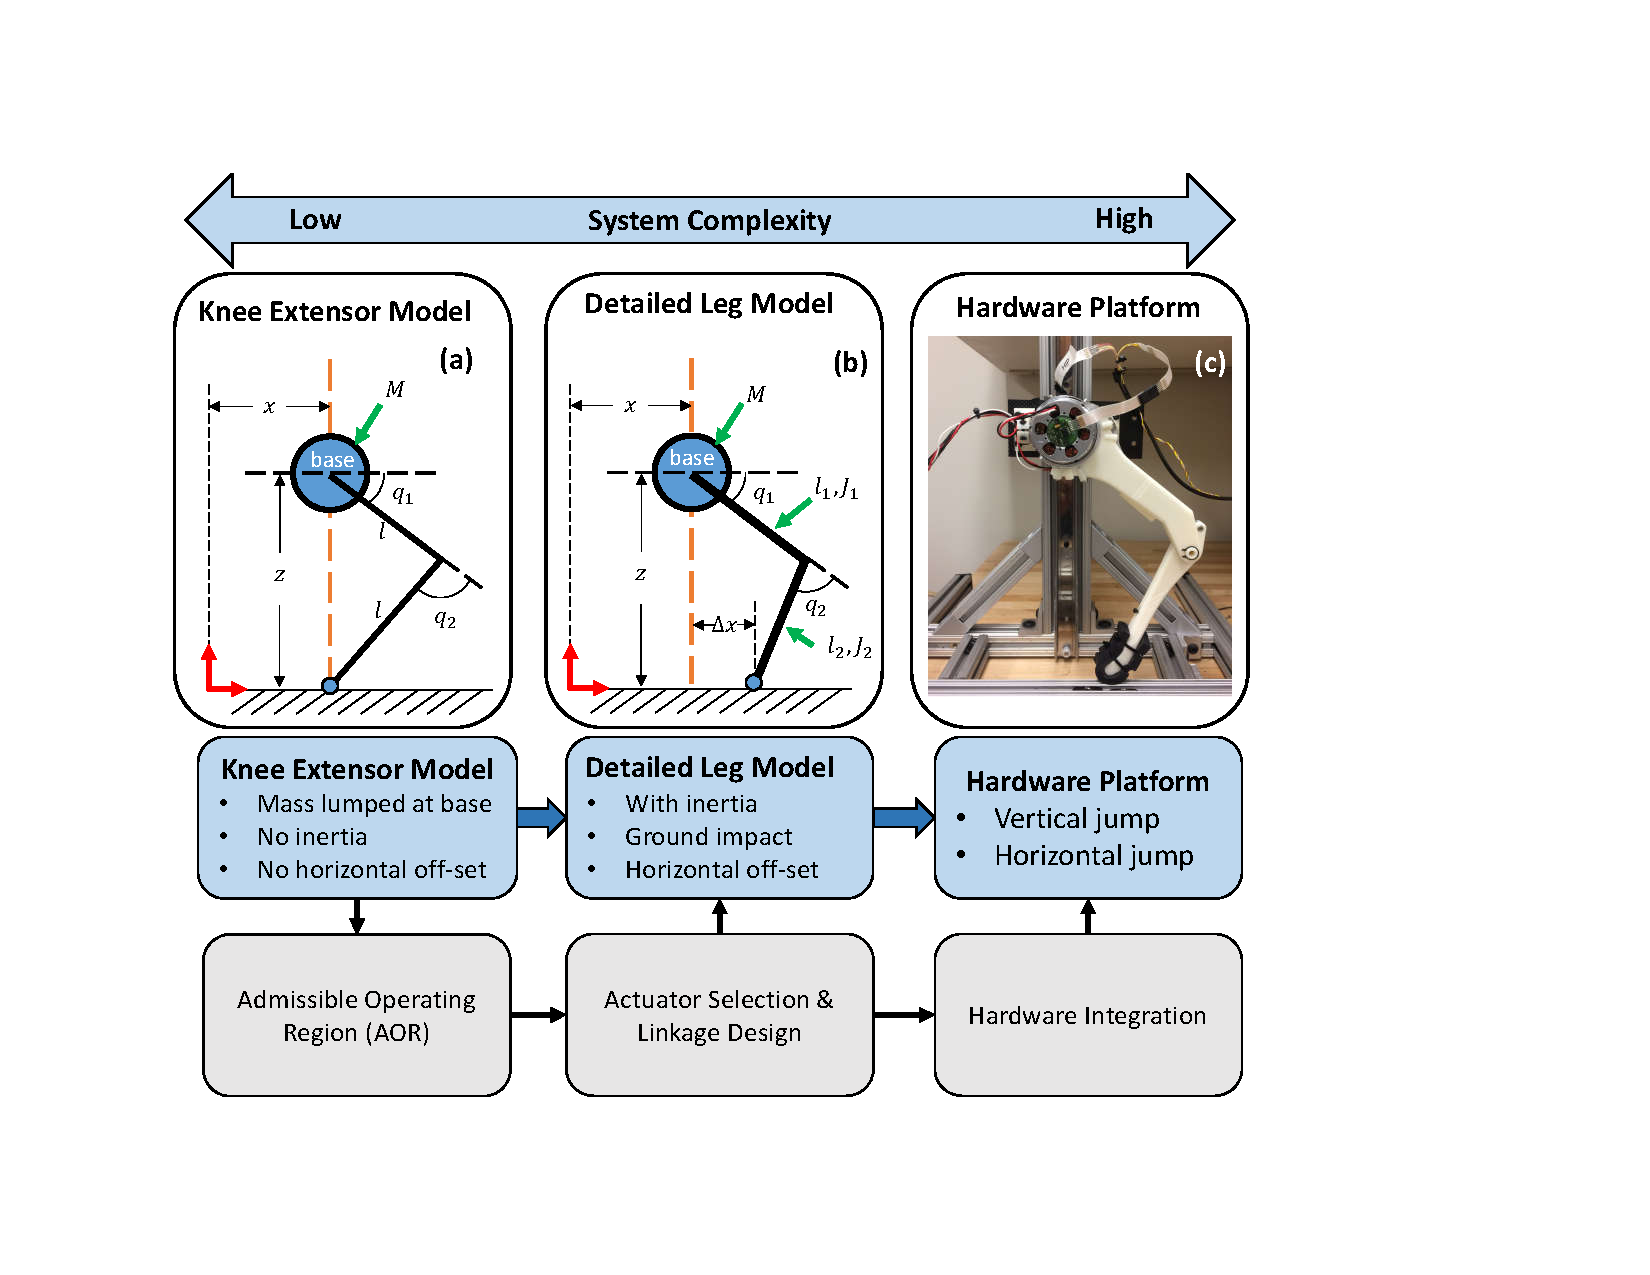
\includegraphics{system_overview.pdf}}
	\caption{Sequential design process for determining design parameters. (a) knee extensor model for motor selection (b) detailed leg model for linkage design and gear ratio choice (c) hardware platform for experiments}
	\label{fig:systemOverview}
\end{figure}

%-------------------------------------------
% ----------Knee Extensor Model----------
\subsection{Knee Extensor Model}
\label{sec:kneeExtensorModel}

The knee extensor model was used to estimate the torque and speed requirements to achieve desirable jumping motions, which provides us with an initial guidance for choosing motor and gearbox. Figure \ref{fig:systemOverview} (a) shows the schematics of the knee extensor model. The model assumes that all masses are lumped at the base to be $M$, which is mounted on a vertical linear rail. Thigh and shank links have an identical length of $l$, while its foot and base are vertically aligned. Hence only the knee joint needs to be actuated to perform vertical jump while the hip joint is not actuated. The vertical height of the base $z$ and joint angles $q_1, q_2$ are shown in Figure \ref{fig:systemOverview}.

The dynamics of this model was formalized as a single point mass accelerated due to ground reaction force (GRF). Ground reaction force was chosen as the control input because it is the only external force in the knee extensor model that could increase the mechanical energy of the system. The equation of motion (EOM) of the system is: $\ddz = \frac{F_z}{M}-g$, where $z$ is the vertical displacement of the base, $F_z$ is the vertical component of GRF, $M$ is the lumped mass at the base and $g$ is the gravitational acceleration. 

%-------------------------------------------
% ----------GRF Parameterized as \Bezier\ Polynomial----------
\subsection{GRF Parameterized as \Bezier\ Polynomial}
\label{sec:BezierPoly}
	
A $5^{th}$ order \Bezier\ polynomial was used to parameterize the GRF profile. The reasons for using \Bezier\ Polynomial to parametrize the ground reaction force is two fold. Firstly, the first and last coefficient of a \Bezier\ polynomial corresponds to the initial and final value of the GRF, which makes it more convenient to anchor GRF to desired values at the initial and final instance; secondly, integration of \Bezier\ Polynomial is a linear operation, which is computationally inexpensive. This property is utilized in integrating the prescribed ground reaction force and integrate to get the velocity trajectory, as shown in Equation \ref{eq:bernstein_integration}, and integrate again to get the position trajectory

The coefficients of \Bezier\ polynomial are assumed to be $[Mg, \alpha_1, \alpha_2, \alpha_3, \alpha_4, 0]$. The first coefficient was set to be the weight of the leg because it is assumed that the leg starts from static equilibrium state, and last coefficient was set as $0$ to ensure a smooth and physically feasible motion at the take-off moment.  

The Bernstein polynomials are defined over [0,1] as:

\begin{equation}
	B_{i,N} = \left(
	\begin{smallmatrix}
	N\\
	i
	\end{smallmatrix}\right)
	x^i(1-x)^{n-i},
	0\leq i \leq N
\end{equation}
where  $\left(
\begin{smallmatrix}
N\\
i
\end{smallmatrix}\right)$
is the binomial coefficients.

Since a \Bezier\ polynomial is the linear combination of a Bernstein polynomial basis\cite{dicsibuyuk2007generalization} defined as,

\begin{equation}\label{eq:bezier}
C_N(s) = \sum_{i=0}^{N}\alpha_i B_{i,N}(s)
\end{equation}

where $\alpha_i$ is the coefficient for the $i^{th}$ Bernstein polynomial $B_{i,N}$, analytical solution for velocity and position could be obtained using the property of the Bernstein polynomial\cite{Doha2011}:

\begin{equation} \label{eq:bernstein_diff}
\frac{d}{ds}B_{i,N}(s)=\frac{N}{T}(B_{i-1,N-1}(s)-B_{i,N-1}(s))
\end{equation}
where $s$ is a point between general time interval $[0, T]$.

Given the initial velocity $\dz_0$, the velocity trajectory in stance phase is a $6^{th}$ order \Bezier\ polynomial with coefficients $\gamma_{(0-6)}$. The linear relationship between force and velocity \Bezier\ coefficient is:

\begin{equation}\label{eq:bernstein_integration}
\frac{6}{T_{st}}\left[
\begin{smallmatrix}
-1 & 1 & 0 & 0 & 0 & 0 & 0 \\
0 &-1 & 1 & 0 & 0 & 0 & 0 \\
0 & 0 &-1 & 1 & 0 & 0 & 0 \\
0 & 0 & 0 &-1 & 1 & 0 & 0 \\
0 & 0 & 0 & 0 &-1 & 1 & 0 \\
0 & 0 & 0 & 0 & 0 &-1 & 1 \\
1 & 0 & 0 & 0 & 0 & 0 & 0 \\
\end{smallmatrix}
\right]
\left[
\begin{matrix}
\gamma_0\\\gamma_1\\\gamma_2\\\gamma_3\\\gamma_4\\\gamma_5\\\gamma_6\\
\end{matrix}
\right]
=
\left[
\begin{matrix}
\left[
\begin{matrix}
0\\\alpha_1\\\alpha_2\\\alpha_3\\\alpha_4\\0\\
\end{matrix}
\right]\frac{1}{M}-g\\
\dz_0\\
\end{matrix}
\right]
\end{equation}
where $T_{st}$ is the stance duration for jumping up.

Similarly, the position trajectory in stance phase could also be integrated by applying the linear operation shown in Equation \ref{eq:bernstein_integration} given initial position $z_0$. At each instance  $t\in[0,T_{st} ]$, the joint angle $q=[q_1,q_2]$ defined in Figure \ref{fig:systemOverview}(a) was solved by inverse kinematics. 

Since the thigh and shank links are assumed to be massless, joint torque $\tau=[\tau_1,\tau_2]$ could be reconstructed using 
\begin{equation}
	\tau=J(q)^T F
\end{equation}

where $\tau_1$ and $\tau_2$ are joint torques for hip and knee joints, $F$ is the ground reaction force, and $J(q)\in R^{2\times 2} $ is the manipulator Jacobian of the foot relative to the hip.

The jumping performance was evaluated by the maximal reachable height $h_{max}$,
 \begin{equation}
 	 h_{max} := h_{to}+\frac{v_{to}^2}{2g}
 \end{equation}

 where $h_{to}$ and $v_{to}$ are the base height and speed at the moment of take-off.

%---------------------------------------------------------------------
% ----------Nonlinear Optimization for Ground Reaction Force----------
\subsection{Nonlinear Optimization for Ground Reaction Force}
\label{sec:nonlOptGRF}

In order to get the optimal ground reaction force profile within actuator limits, an optimal control problem was formulated and solved using nonlinear optimization:
\begin{equation}\label{eq:path_constraints}
\begin{aligned}
\min&~~~~~~~~~~-h_{max}\\
s.t.&~~~~~~~q_{lb}\leq q \leq q_{ub}\\
&~~~~~~~\dq_{lb}\leq \dq \leq \dq_{ub}\\
&~~~~~~~\tau_{lb}\leq \tau \leq \tau_{ub}\\			 	
\end{aligned}
\end{equation}
where $q_{lb}$, $q_{ub}$ are the lower and upper bounds for joint angles; $\dq_{lb}$, $\dq_{ub}$ for angular velocity; $\tau_{lb}$, $\tau_{ub}$ for joint torques.  

Dynamics was discretized at $N$ sampling points to search for optimal variable values. Joint angle $q$ and angular velocity $\dq$ were discretized at the sampling points. Motor's maximal speed and torque constraints were imposed at each sampling point as inequality constraints.

The optimization variables are chosen as follows:
\begin{equation}\label{eq:opt_var_knee}
x_{opt} = [z_0, \alpha_{(1-4)}, T_{st}, q_{(1-N)}, \dq_{(1-N)}]
\end{equation}
where $x_{opt}$ is the vector of optimization variables for stance phase; $z_0$ is the base's vertical initial position; $\alpha_{(1-4)}$ are the \Bezier\ polynomial coefficients of ground reaction force; $T_{st}$ is the total stance time; $q$ is the vector of joint angles and $\dq$ is the vector of joint velocities at all the sampling points.

Equality constraints were imposed to satisfy forward kinematics:

\begin{equation}
\label{eq:kin_position}
rot(q_1)
\left[\begin{matrix}
l\\0
\end{matrix}\right]
+
rot(q_1+q_2)\left[\begin{matrix}
l\\0
\end{matrix}\right]
+
\left[\begin{matrix}
0\\z
\end{matrix}\right]
=0
\end{equation}

\begin{equation}
\label{eq:kin_velocity}
J(q)\dq+\left[\begin{matrix}
0\\ \dz
\end{matrix}
\right]
=
\left[\begin{matrix}
0\\0
\end{matrix}\right]
\end{equation}
where $rot\in SO(2)$ is the rotation matrix. $z$ and $\dz$ are the vectors of height and velocity of the base at each sampling point using Equation \ref{eq:bernstein_integration}.


MATLAB's $fmincon$ function was used to search for local optimal solutions. The parameters for the knee extensor model is chosen as follows: mass $M = 0.66~kg$, link length $l=0.12~m$. 100 simulation runs were executed over 10 different maximal motor speed ($\omega_{max}$ from 23 rad/s to 37 rad/s) and maximal torque ($\tau_max$ from 6.2 Nm to 9.7 Nm) constraints, then the maximal achievable height $h_{max}$ is plotted as the third axis against $\tau_{max}$ and $\omega_{max}$. As shown in Figure \ref{fig:hmax_pcolor}, the maximal achievable height increases as the upper limit for speed and torque increases. The level curves shows that $h_{max}$ could reach as high as 0.8 m theoretically with the effective actuator torque of 9.7 Nm and actuator speed of 37 rad/s.

The advantage of this method is that it decoupled the study of jumping to two decoupled problems. In terms of dynamics, it treats the leg as a point mass accelerated due to ground reaction force and gravity; in terms of kinematics, it assumes two link kinematics chain for leg topology. After imposing equality constraints which bridges the error between kinematics as shown in Equations \ref{eq:kin_position} and Equation \ref{eq:kin_velocity}, the problem is tackled in a way that avoids the problem of singularity in the search of optimization variables.


%-----------------------------------------------
% ----------Admissble Operating Region----------
\subsection{Admissble Operating Region}
\label{sec:AOR}

\begin{figure}
	\centering
	\resizebox{1.0\linewidth}{!}{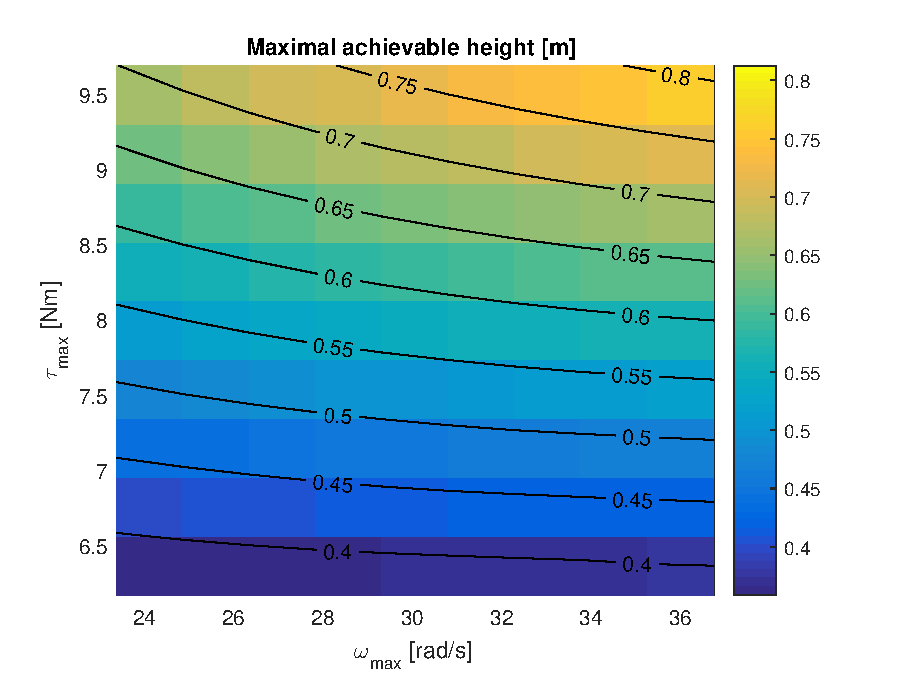
\includegraphics{hmax_pcolor.eps}}
	\caption{Maximal achievable height for specific torque and speed limit. The x-axis corresponds to maximal angular velocity of the actuator, the y-axis corresponds to maximal torque of the actuator, and the depth represents the maximal achievable height of a jump}
	\label{fig:hmax_pcolor}
\end{figure}

\begin{figure}
	\centering
	\resizebox{0.8\linewidth}{!}{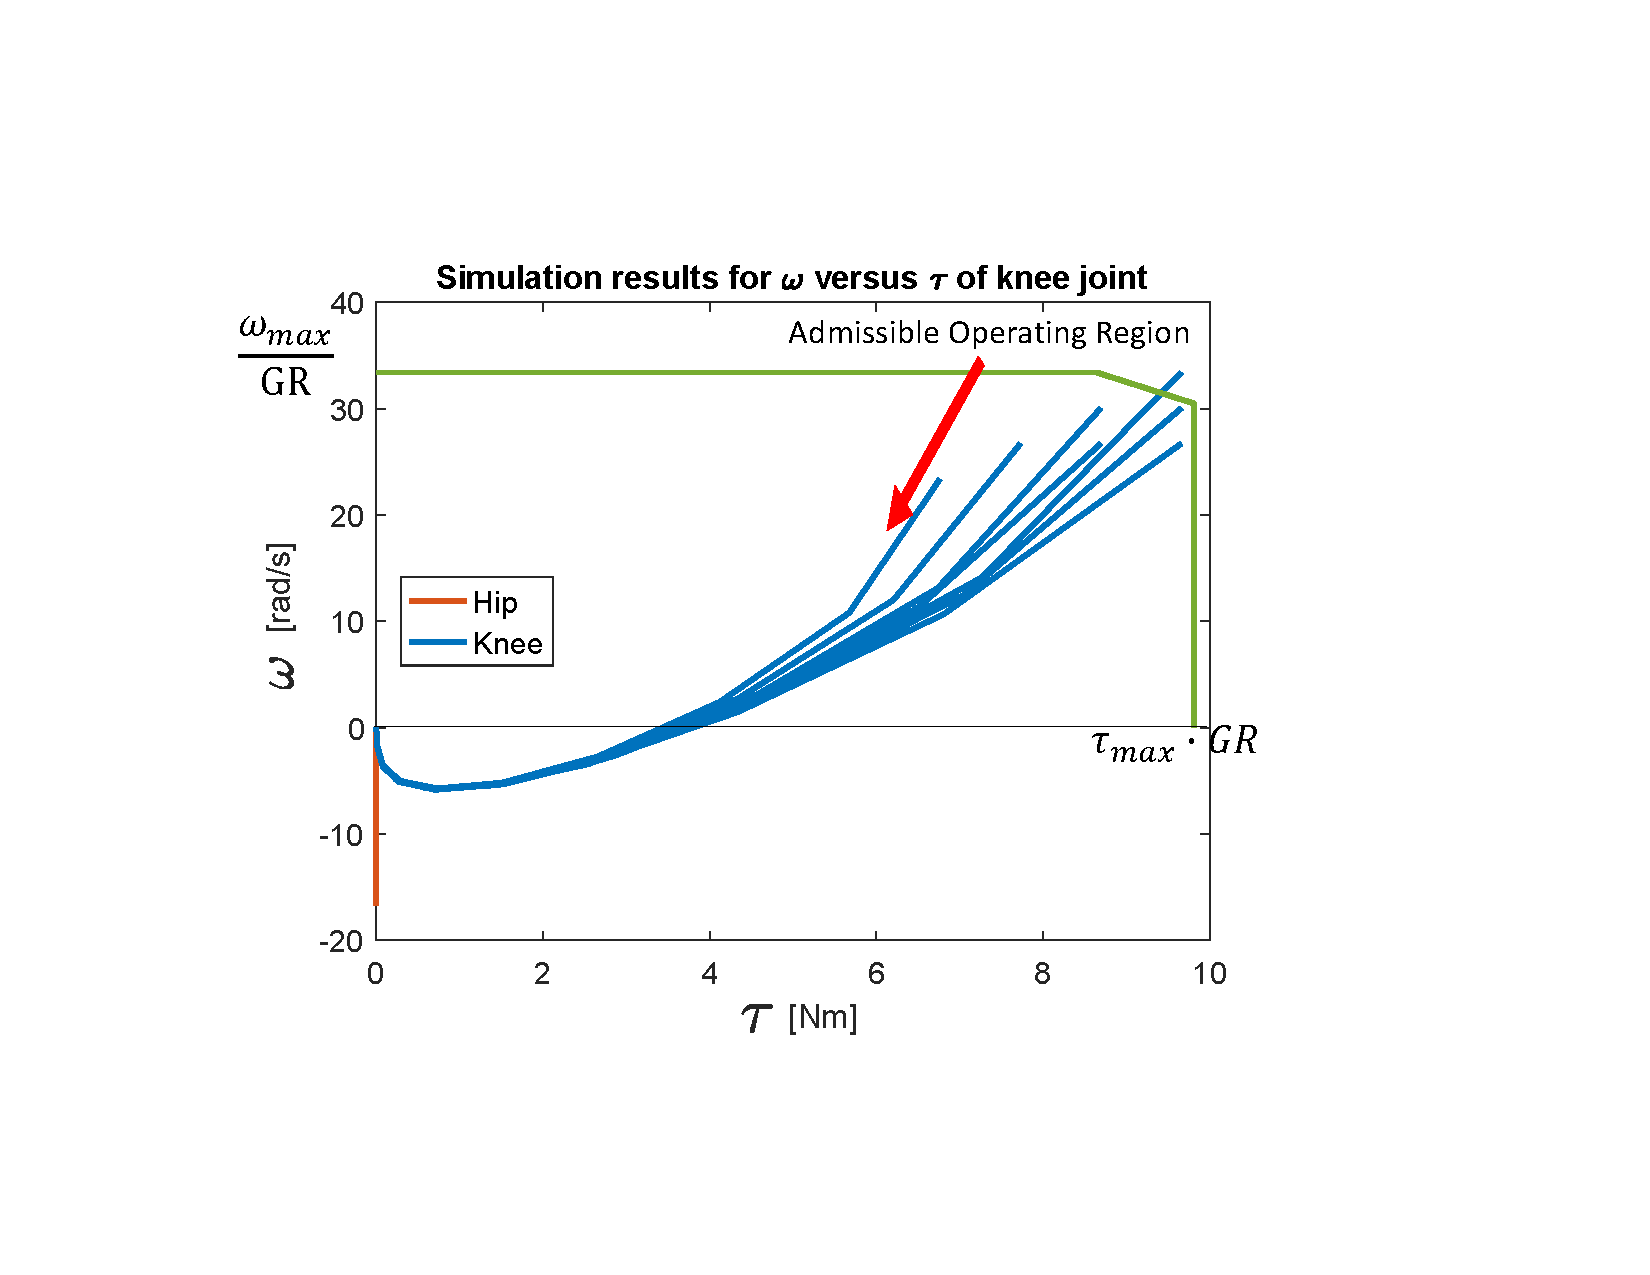
\includegraphics{AOR.pdf}}
	\caption{The Admissible Operating Region (AOR) formed by the torque and angular speed trajectories from the one hundred knee extensor model simulations. A typical motor's speed-torque curve scaled by gear ratio of 23:1 is plotted in green curve. Hip motor acts as a passive joint throughout the jumping up phase.}
	\label{fig:AOR}
\end{figure}

 In general, Admissible Operating Region (AOR) is defined as the area in the torque-speed plane enclosed by the Leg's torque-speed trajectory in performing certain task, as is shown in Figure \ref{fig:AOR}. The motions corresponding to the enclosed AOR region are admissible to the actuator. It is a projection of dynamic motion to the torque-speed domain of the actuators. It is a lumped quantity which treats the motor and gearbox as a unity instead of separating the characteristics of both. The contribution of the proposition of AOR is that it captures the essence of robot motion generation, and bridges between motor dynamics, and workspace dynamics. Furthermore, it could be used in the early stage of design by projecting workspace dynamics to actuator's speed-torque space, before the choice of motor and transmission design is determined. 
 
 \subsubsection{Scaling Effect of Gear Ratio}
 \label{sec:GR_scale_effect}
 
 The analysis of AOR takes motor and gearbox as a whole entity. Since AOR is determined by desired motion, it does not change with gear ratio, hence it is independent of actuator and gearbox choices. What the gear ratio could scale is the motor characteristic curve. Shown as the green curve in Figure \ref{fig:AOR}, the original speed-torque curve of this specific motor is scaled by gear ratio to enclose more of the AOR. Namely, the maximal motor speed $\omega_{max}$ is scaled down to $\omega_{max}/GR$, and the maximal motor torque $\tau_{max}$ is multiplied to $\tau_{amx}GR$. Geometrically speaking, the motor characteristic curve has become lower and wider. 
 
 \subsubsection{Zero Torque at the Hip Joint}
 
 Multiple simulation results from Section \ref{sec:nonlOptGRF} is plotted in Figure \ref{fig:AOR} shown as blue curves. Note that the torque requirement for Hip motor shown in red line is always zero. This result conforms to our formulation of the Knee Extensor Model, which assumes the foot is located directly below the hip point.
 
 \end{comment}
 
 



\chapter{Design Principles for Dynamic Legged Robots}

%%%%%%%%%%%%%%%%%%%%%%%%%%%%%%%%%%%%%%%%
%          Transmission
%%%%%%%%%%%%%%%%%%%%%%%%%%%%%%%%%%%%%%%%

\section{Transmission Design}
\label{sec:transmissionDesign}

The actuator design philosophy is to make high power actuators with the capability of interacting with the environment. Namely, the actuator should not be stiff as the heavily geared motors, which are widely used in industrial robots. Instead, it should be back-drivable meaning that the torque applied at the output shaft should be felt at the input shaft. The benefits are threefold, firstly, back-drivability prevents geatboxes from being damaged by external forces; second, it allows for proprioceptive sensing\cite{Seok2012}; thirdly, allows for fast dynamics in legged locomotion.

After the motor selection and gear ratio is determined from previous sections, focus was put on how to design the transmission system so that it can achieve the desired gear ratio while satisfying dimensional constraints.

\subsection{Transmission Design Comparison}
\label{sec:transmissionComparison}

\textbf{Harmonic drive} is composed of the wave generator, flexspline and circular spline. It could provide high gear ratio typically between 30:1 to 200:1 with zero backlash. Harmonic drive is employed by the quadrupedal robot starlETH\cite{Hutter2013} and the bipedal robot ATRIAS\cite{Hubicki2016}. However, harmonic drive is not back-drivable, which contradicts with our design paradigm.

\textbf{Cycloidal gearbox} has very low backlash and high torsional stiffness. It can operate quietly and withstand shock load. Bipedal robot Cassie uses cycloidal gearbox as the transmission. The drawback of cycloidal gearbox is that it requires customizing high precision parts.

\textbf{Single stage planetary gearbox} has high efficiency and the load could be distributed between planet gears, and standard gears are widely available at low cost. Nevertheless, no gear combination could provide the desired gear ratio for the given dimensional limitation with pitch of 0.4.

\textbf{Compound planetary gearboxes} have the benefits of single stage planetary gearboxes while providing more compact design for there are two stages for the planet gear. There are a range of gear teeth selection for the given dimensional limits. It is adopted as the transmission system design considering the dimensional limit and gear ratio requirement of the motor design.

\subsection{Compound Planetary Gearbox Design}
\label{sec:compoundGearBox}

\begin{figure}
	\centering
	\resizebox{1.0\linewidth}{!}{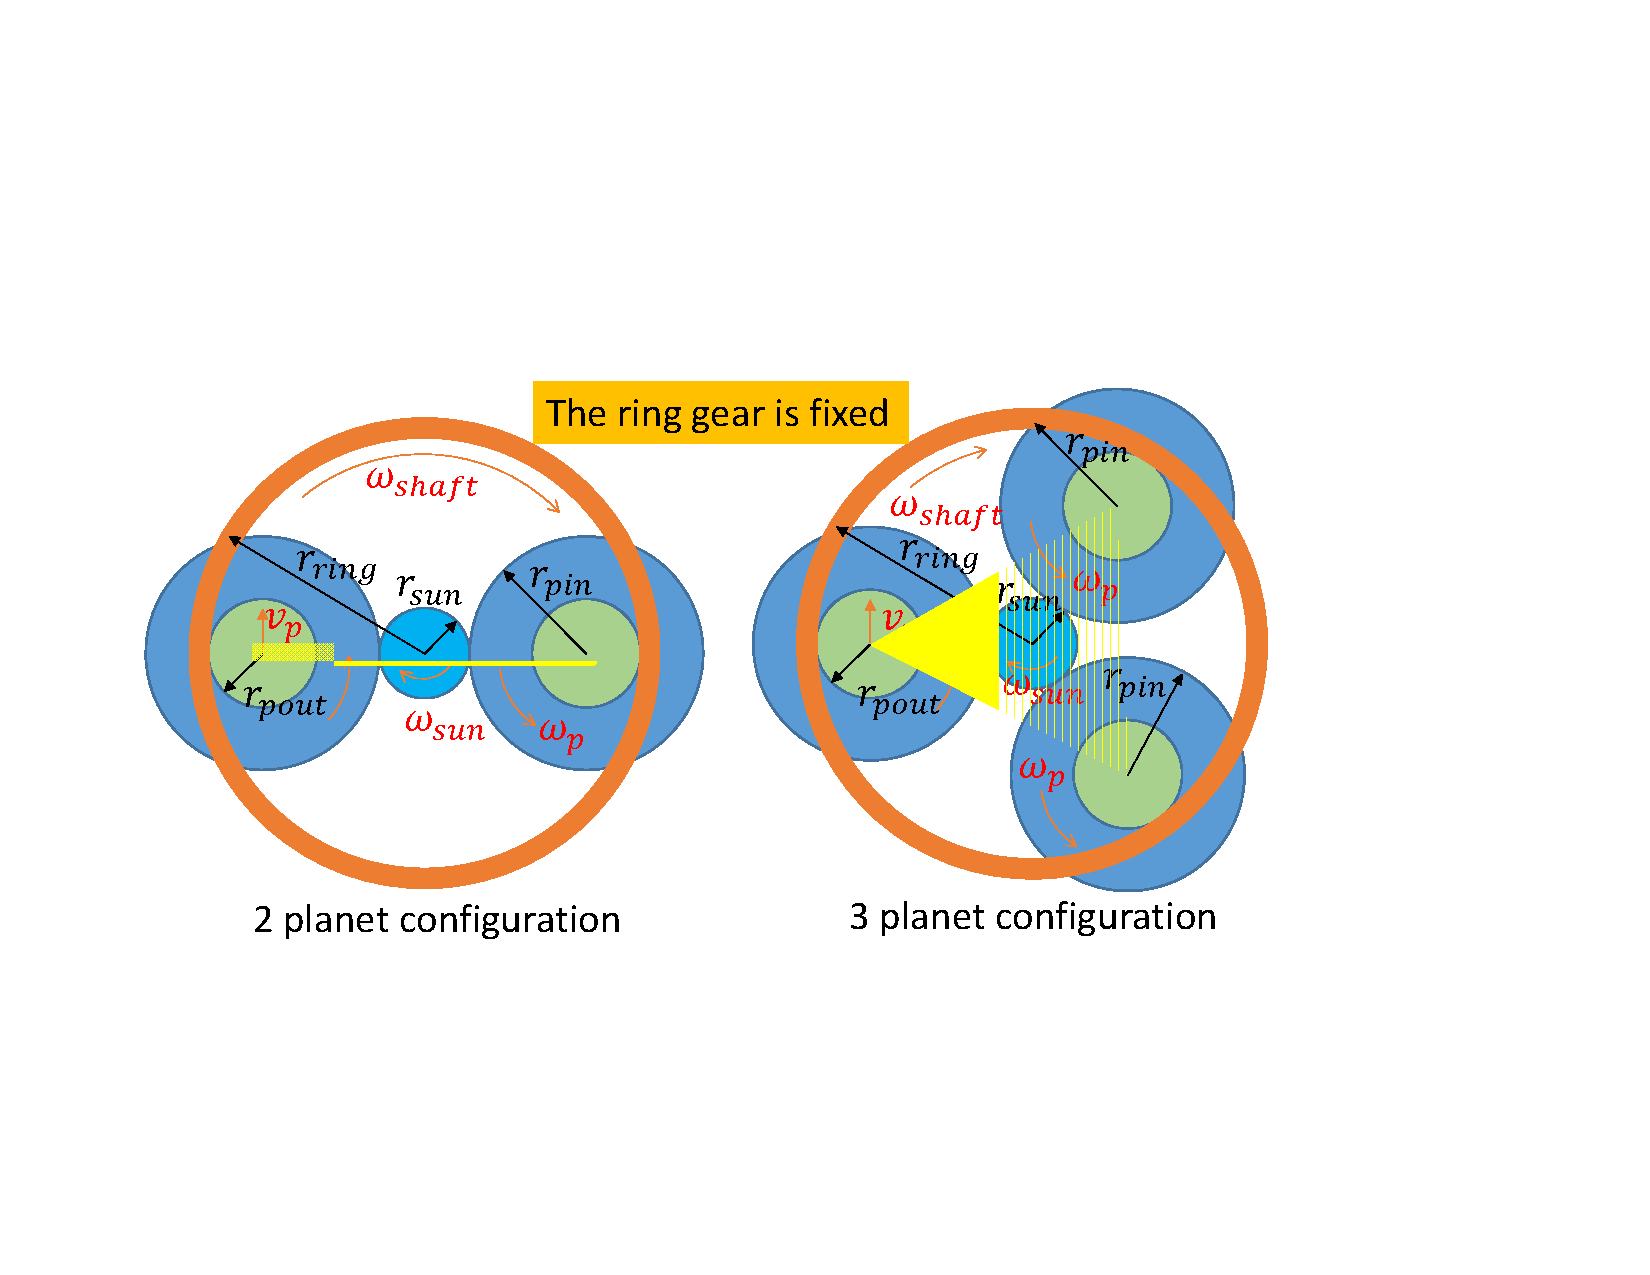
\includegraphics{planetaryGearbox.pdf}}
	\caption{Schematics of Compound Planetary Gearbox Configurations. (left) 2 planet configuration, (right) 3 planet configuration}
	\label{fig:planetaryGearbox}
\end{figure}

The objective of compound planetary gearbox design is to achieve desired gear ratio within dimensional constraints imposed by motor selection. In order to derive the gear ratio for given gear teeth number, a schematics of the two-stage compound planetary gearbox is used as shown in Figure \ref{fig:planetaryGearbox}. For given gear teeth numbers, both configurations in Figure \ref{fig:planetaryGearbox} are equivalent. Some assumptions for this analysis is posed here: 

\begin{enumerate}
	\item The sun gear located at the center is the input.
	\item The output shaft shown as yellow transparent shape is the output.
	\item The output shaft is connected to the axes of all the planet gears.
	\item The sun gear is meshed with input planet gears.
	\item The ring gear is meshed with output planet gears.
	\item The ring gear is fixed.
\end{enumerate}

Velocity equivalence is used to calculate the gear ratio.
\begin{eqnarray}
\omega_{sun} r_{sun} =& v_p + \omega_p r_{pin}\\
v_p =& \omega_{p} r_{pout}\\
\omega_p =& \frac{\omega_{sun}r_{sun}}{r_{pout}+r_{pin}}\\
\omega_{shaft} =& \frac{\omega_{p}r_{pout}}{r_{sun}+r_{pin}}
\end{eqnarray}
where $\omega_{shaft}$ is the angular velocity of the output shaft and the rest of the variable definitions could be found in Table \ref{tab:varDefGearbox}.

Therefore, the gear ratio of a compound planetary gearbox could be formulated as:
\begin{equation}
GR = \frac{\omega_{sun}}{\omega_{shaft}} = \frac{(r_{pout}+r_{pin})(r_{sun}+r_{pin})}{r_{sun}r_{pout}} = \frac{(N_{pout}+N_{pin})(N_{sun}+N_{pin})}{N_{sun}N_{pout}}
\end{equation}

\begin{table}[bp]
	\centering
	\caption{Variable Definition for Gear Ratio Calculation}
	\begin{tabular}{lcccc}\hline\hline
		& Sun gear		& Input planet	& Output planet	& Ring gear \\ \hline
		Pitch diameter	& $r_{sun}$	   	& $r_{pin}$		& $r_{pout}$	& $r_{ring}$\\
		Angular velocity& $\omega_{sun}$& $\omega_{p}$	& $\omega_{p}$	& N/A		\\
		Linear velocity	& N/A			& $v_p$			& $v_p$			& N/A		\\
		Teeth number	& $N_{sun}$		& $N_{pout}$	& $N_{pout}$	& $N_{ring}$\\ \hline
	\end{tabular}
	\label{tab:varDefGearbox}
\end{table}

The planetary gearbox shown in Figure \ref{fig:gearbox} utilizes two-stage compound planet gears to provide desired gear ratio while satisfying the dimensional constraints imposed by motor selection. 

The constraints for choosing teeth numbers are listed as follows:

\begin{enumerate}
	\item The teeth number of sun gear ($N_{sun}$) and ring gear ($N_{ring}$) could both be divided by the number of planet gears.
	\item The pitch circles of sun gear and planet gears, as well as that of planet gears and the ring gear should be externally tangent, 
	
	i.e. $r_{ring}=r_{sun}+r_{pin}+r_{pout}$ or $N_{ring}=N_{sun}+N_{pin}+N_{pout}$.
	\item The gear ratio $GR$ should be within the range of 22 - 25.
	\item The radius of the gearbox should be less than 25 mm, 
	
	i.e. $Max[r_{ring},r_{sun}+2r_{pin}]<12.5 mm$
	\item The teeth number for sun gear $N_{sun}$ should be no less than 6. Other wise the meshing would be problematic because the profile of gear teeth would be distorted too much.
\end{enumerate}

On top of the constraints, some practical issues were also considered in choosing gear teeth. Ideally, the phase difference between two stages of the planet gears should be the same. However, in compound gear manufacturing, the phase differnce could not be well maintained. To solve this problem, the planet gear teeth combination was chosen to be 16/53, which only share the common factor of 1. This choice provides tunable backlash with $2.1^{\circ}$ increment in the gearbox assembly. This is very similar to the working principle of a mechanical caliper, which uses two scales (main scale and vernier scale) with small difference to achieve high precision.

A large number of teeth combinations were enumerated taking into account all the constraints. The optimal gear teeth choice emerged as $N_{sun} = 12; N_{pin} = 53; N_{pout} = 16; N_{ring} = 81$ and the gear ratio is 23.3594.

All gears are custom made by \textit{HPC Gears Ltd} with 0.4 pitch and pressure angle of $20^{\circ}$.

%%%%%%%%%%%%%%%%%%%%%%%%%%%%%%%%%%%%%%%%
%          Leg Topology Comparison
%%%%%%%%%%%%%%%%%%%%%%%%%%%%%%%%%%%%%%%%
\section{Leg Topology Comparison}
\label{sec:LegComparison}
The full leg module will have three degrees of freedom (DOF) in order to achieve agile 3D maneuver. Three leg topologies, namely, open-serial chain, parallel five-bar and symmetric five-bar are analyzed in terms of workspace, force production and proprioceptive sensing. For simplicity, the abduction/adduction (ABAD) DOF is neglected and only motion in the 2-D hip-knee plane is analyzed. The analysis is based on the linkage analysis of Minitaur\cite{Kenneally2016}, but extended its analysis to negative $\delta$ value. Also, radial and lateral force, velocity and proprioceptive sensitivity are the three main concern in this section. In this section, all the analysis is based on the assumption of massless links, that is, no linkage mass or inertia is considered. This is valid in real application because the majority of mass is taken by actuators, which could be placed at the base of the link and transmit power via some kind of power transmission system like linkage, chain or belt. Therefore, linkage mass is relatively light compared to the body or even less than 10\% of the total mass, as shown in the MIT Cheetah design\cite{Hae-WonPark1PatrickM.Wensing22015}.

\begin{figure}
	\centering
	\resizebox{0.8\linewidth}{!}{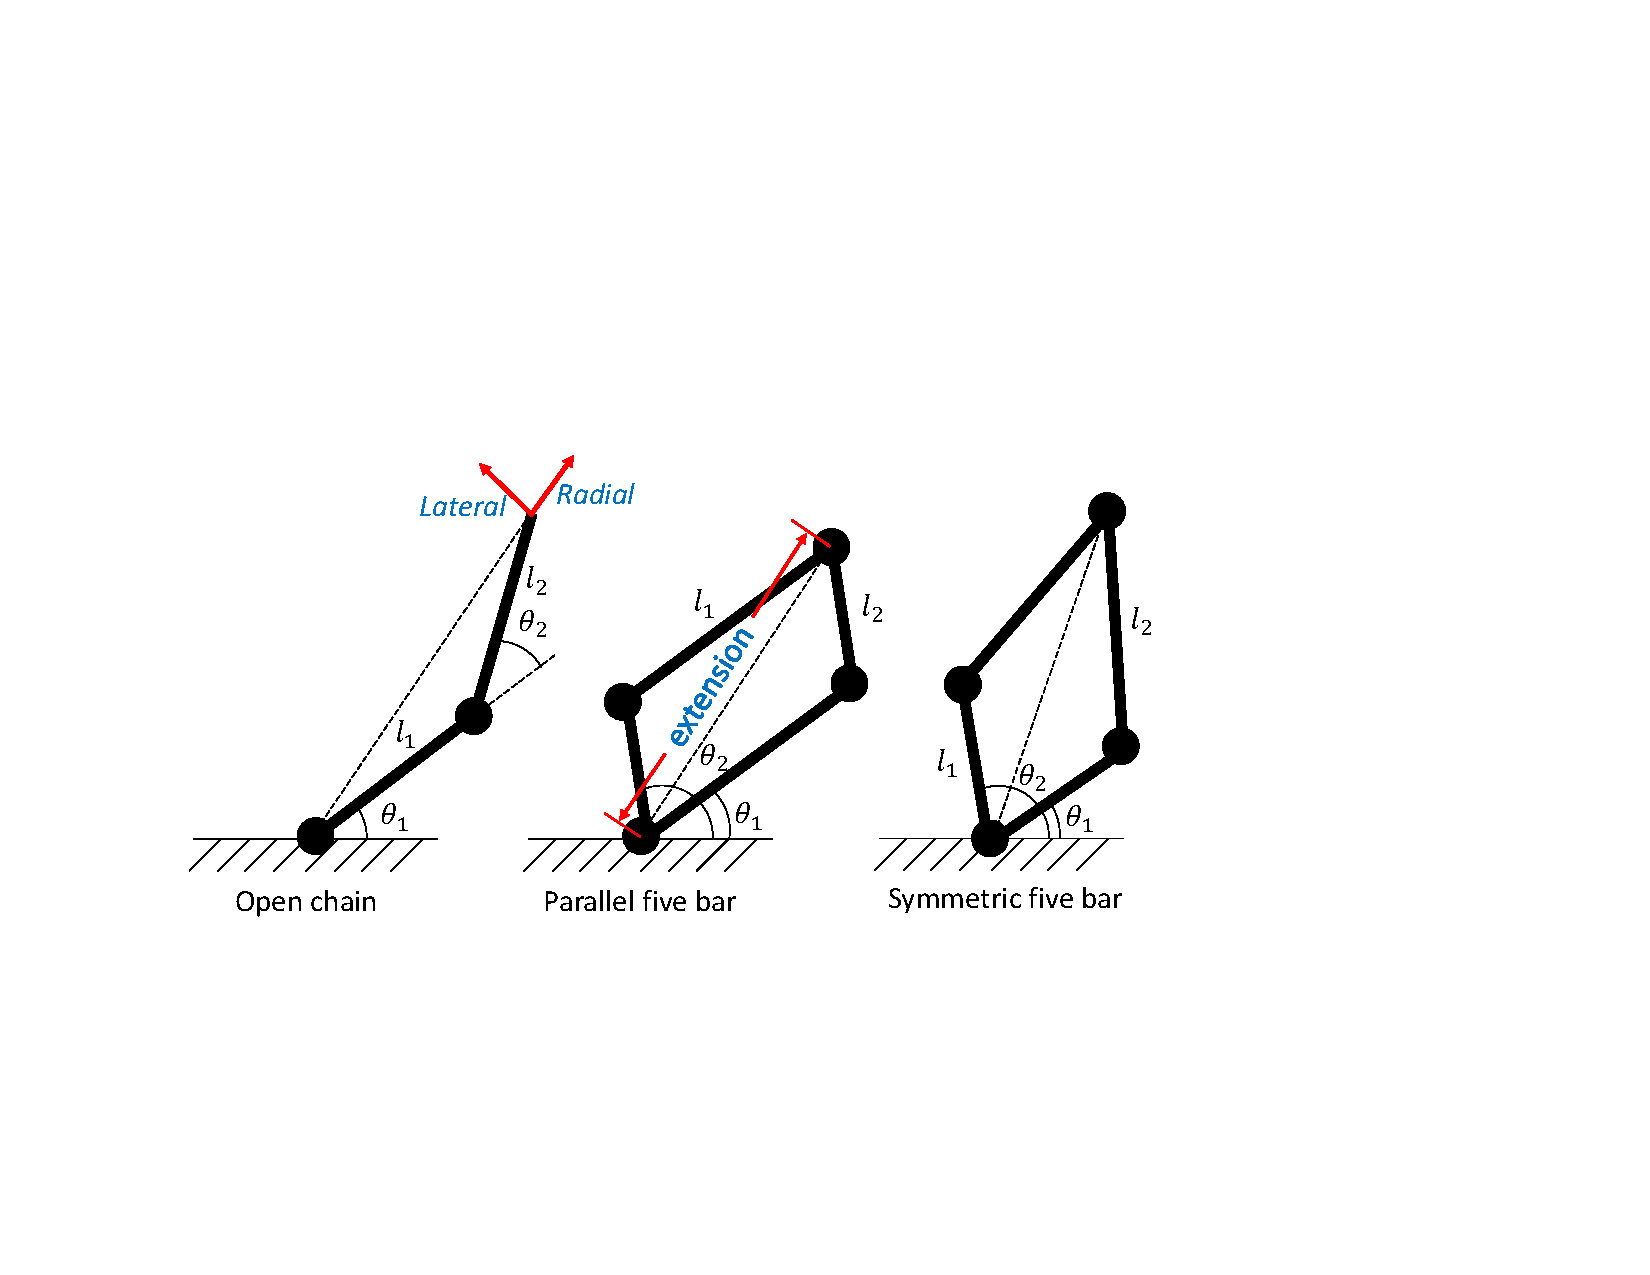
\includegraphics{linkages.pdf}}
	\caption{Three typical linkage topologies (a)Open-serial chain (b)Parallel five-bar (c)Symmetric five-bar. The design variable is $\delta$ and the workspace variable is the leg's radial extension}
	\label{fig:linkages}
\end{figure}

%-------------------------------------------
% ----------Workspace----------
\subsection{Workspace}
\label{sec:workspace}
 	For the three candidate leg topologies shown in Figure \ref{fig:linkages}, the workspace is an annulus, which could be characterized by maximum radius $r_{max}$ and minimum radius $r_{min}$ of the annulus. The design space is defined as:
 	\begin{equation}
 		\delta=\frac{r_{min}}{r_{max}}
 	\end{equation}
 	where $r_{max} = l_1 + l_2$ and $r_{min} = l_1 - l_2$, and $l_1,~l_2$ are the lengths of the first and second links shown in Figure \ref{fig:linkages}. Notice that here $\delta \in (-1,1)$, which means $l_1$ chould be either longer or shorter than $l_2$, which serves as an extension to the analysis presented in \cite{Kenneally2016}.
 	
%-------------------------------------------
% ----------Sweep Volume----------
\subsection{Sweep Volume}
\label{sec:sweepVolume}
	For quadrupedal robot application, sweep volume is also another important factor to consider in linkage design. Large sweep volume is not desirable because the four limbs of a quadrupedal robot are close to each other and the workspace would be decreased if the sweep volume is large. In addition, when interacting with unstructured terrain, large sweep volume increases the possibility of tripping and colliding. For example, when a robot is climbing upstairs, the leg sweep volume should stay clear of the stairs to avoid collision. In out door environment where there are debris and fabric that could easily tangle the robot, a slimmer and compact leg design would be more advantageous. Hence minimized sweep volume is favorable for quadrupedal robot leg design.

%-------------------------------------------
% ----------Force Production----------
\subsection{Force Production}
\label{sec:forceProduction}

	Manipulability ellipsoids are used to characterize a robot arm's ability to move in certain configuration\cite{Lynch2016}. In the following sections, manipulability ellipsoids of force production, velocity production and proprioceptive sensitivity are utilized to present a manipulator's mechanical performance.
	
	Force production ellipsoid characterizes how unit joint torque from motors will reflect as end-effector forces. Solution to equation \ref{eq:force_production} forms the Force production ellipsoid. The major and minor axes of the force production ellipsoid represent the end-effector's strongest and weakest ability to produce force at the respective directions.

	\begin{equation}\label{eq:force_production}
		E_{force} := \{F | F^T J J^T F = ||\tau|| , ||\tau||=1\}
	\end{equation}

	Radial/Lateral force production is defined as the end-effector force in radial/lateral directions given unit joint torque input. Figure \ref{fig:force_openChain} \ref{fig:force_fiveBar} \ref{fig:force_symm} show how force production ability changes over $extension$ and $\delta$.
	
	
	\begin{figure*}
		\centering
		\resizebox{\linewidth}{!}{\includegraphics{egLink_force_ellip.pdf}}
		\caption{Force production in radial direction for an example linkage design of Open-chain, Parallel five-bar and Symmetric five-bar}
		\label{fig:egLink_force_ellip}
	\end{figure*}
	
	\begin{figure*}
		\centering
		\resizebox{0.7\linewidth}{!}{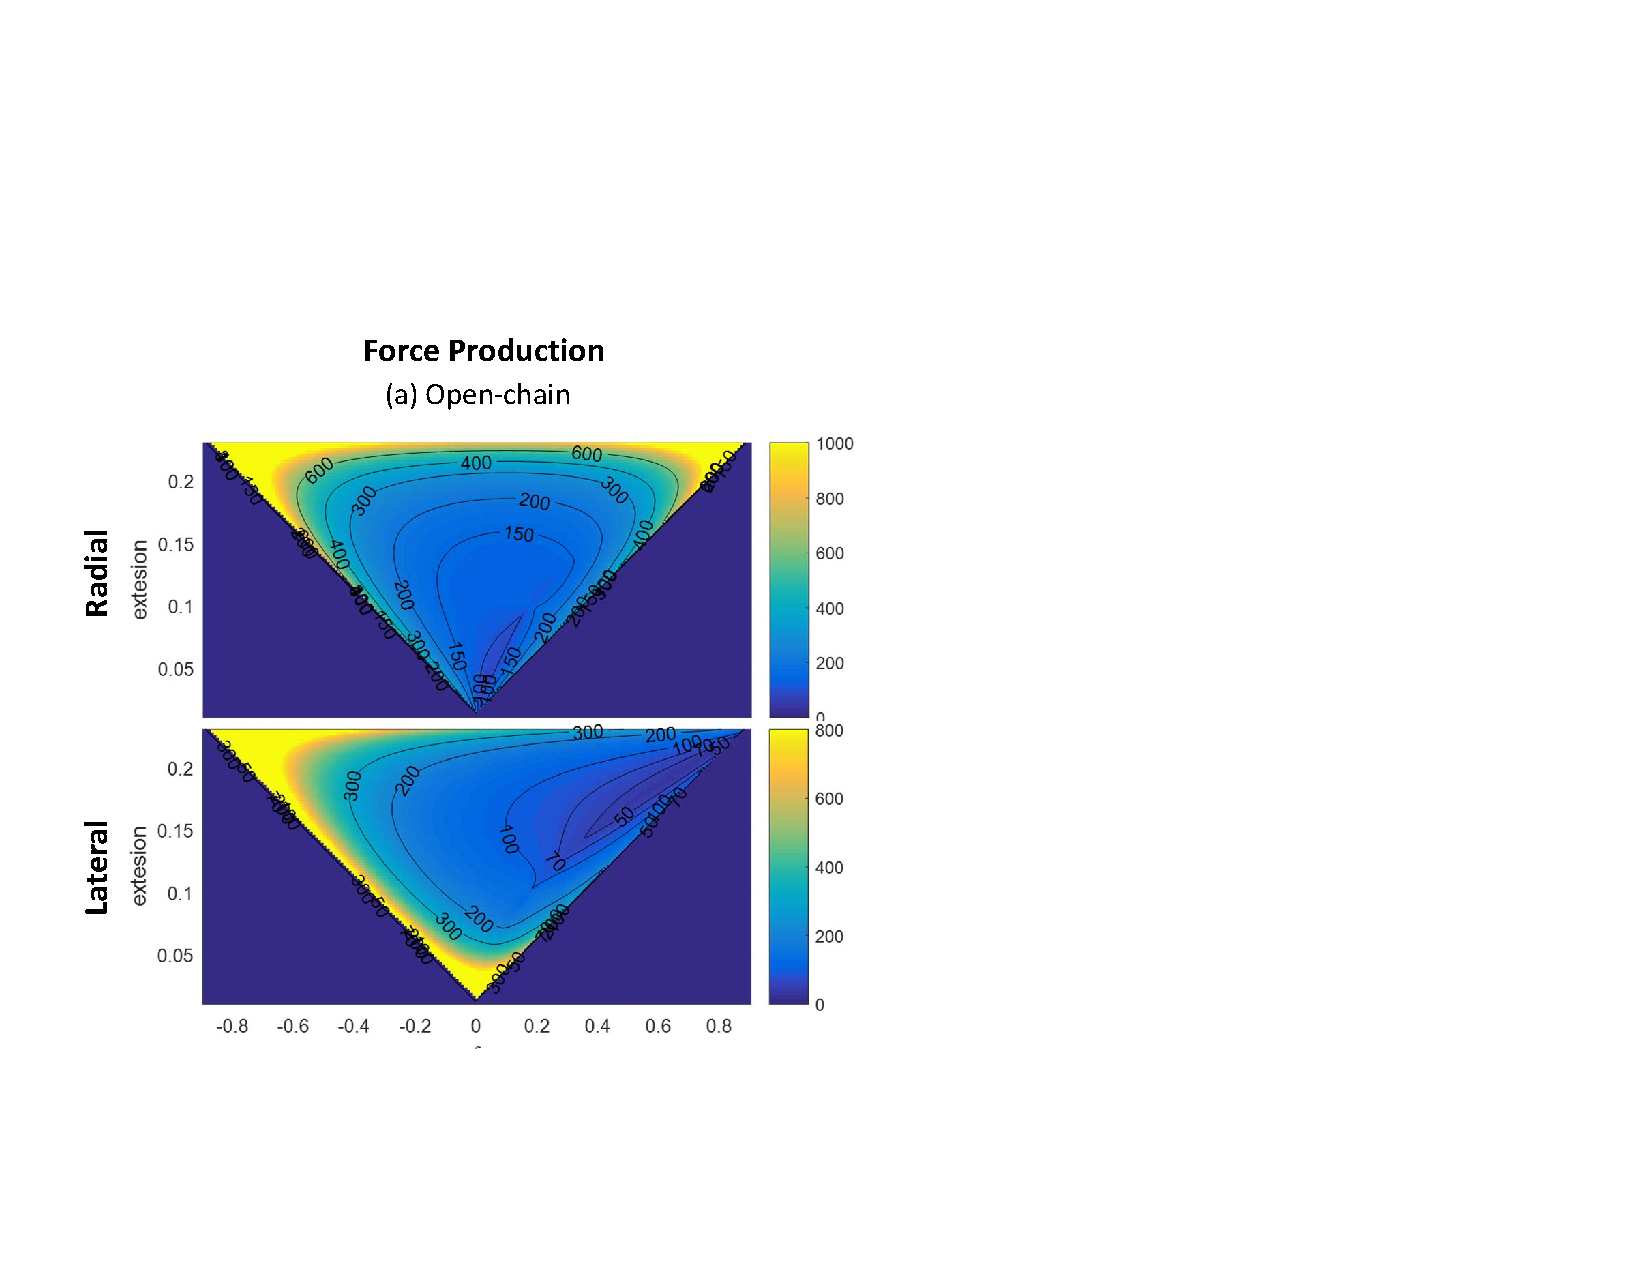
\includegraphics{force_openChain.pdf}}
		\caption{Force production in radial and lateral directions for open chain design}
		\label{fig:force_openChain}
	\end{figure*}

	\begin{figure*}
		\centering
		\resizebox{0.7\linewidth}{!}{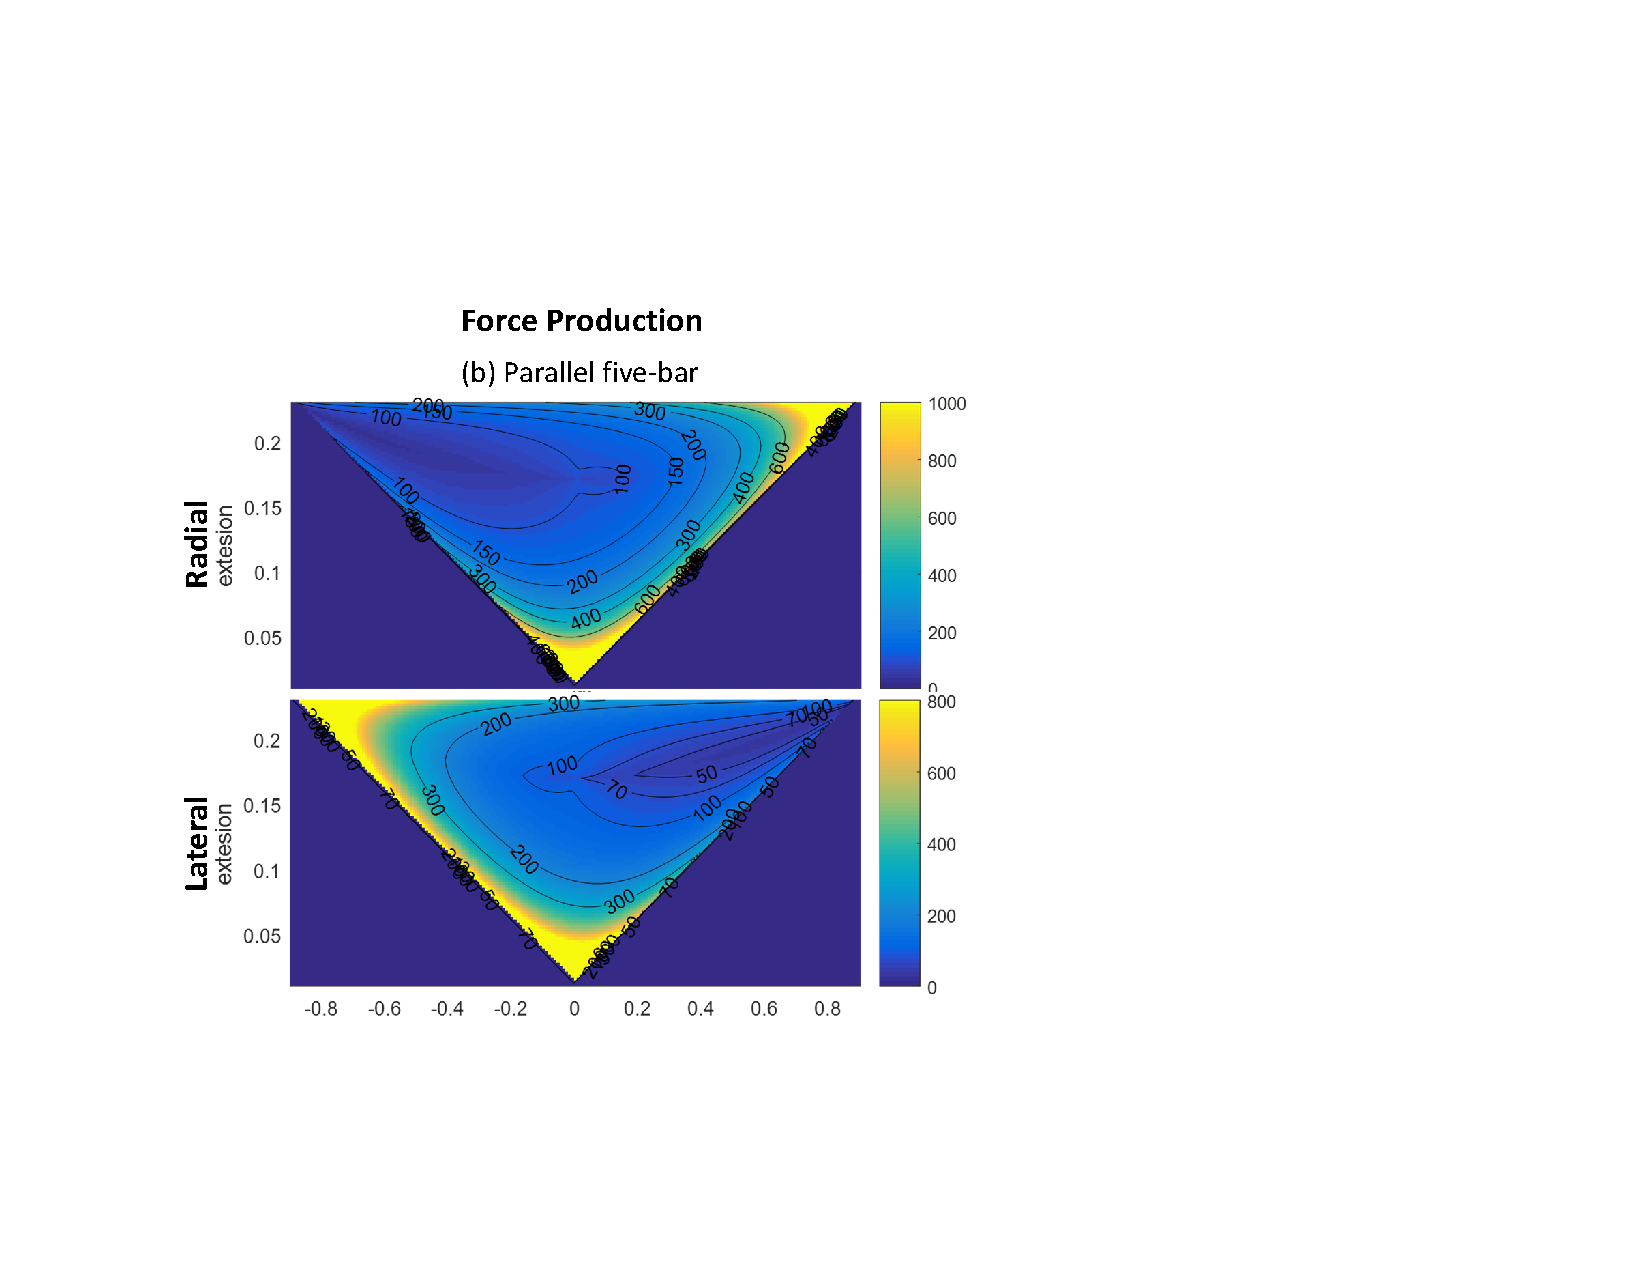
\includegraphics{force_fiveBar.pdf}}
		\caption{Force production in radial and lateral directions for parallel five-bar design}
		\label{fig:force_fiveBar}
	\end{figure*}

	\begin{figure*}
		\centering
		\resizebox{0.7\linewidth}{!}{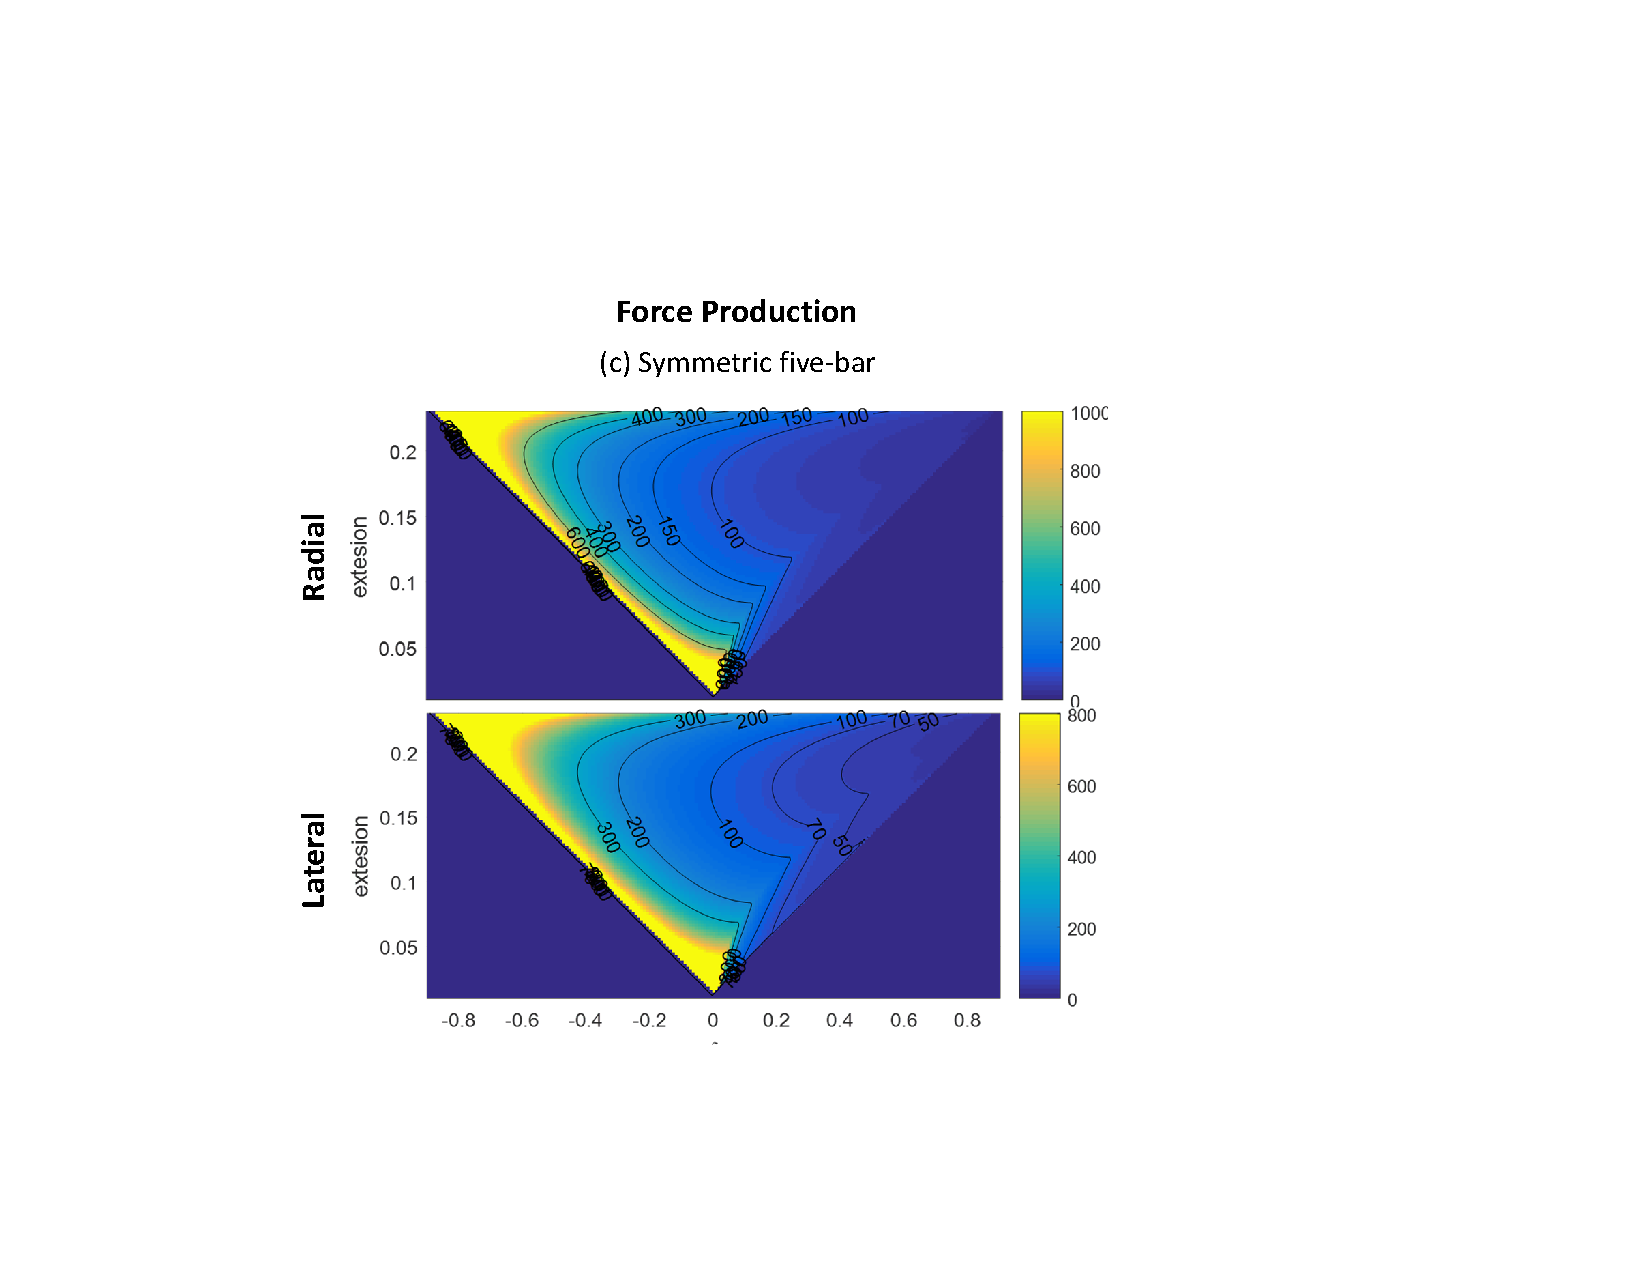
\includegraphics{force_symm.pdf}}
		\caption{Force production in radial and lateral directions for symmetric five-bar design}
		\label{fig:force_symm}
	\end{figure*}

%-------------------------------------------
% ----------Velocity Production----------
\subsection{Velocity Production}
\label{sec:velcotyProduction}

	\begin{figure*}
		\centering
		\resizebox{\linewidth}{!}{\includegraphics{egLink_vel_ellip.pdf}}
		\caption{Velocity production in radial direction for an example linkage design of Open-chain, Parallel five-bar and Symmetric five-bar}
		\label{fig:egLink_vel_ellipp}
	\end{figure*}

	\begin{figure*}
		\centering
		\resizebox{0.7\linewidth}{!}{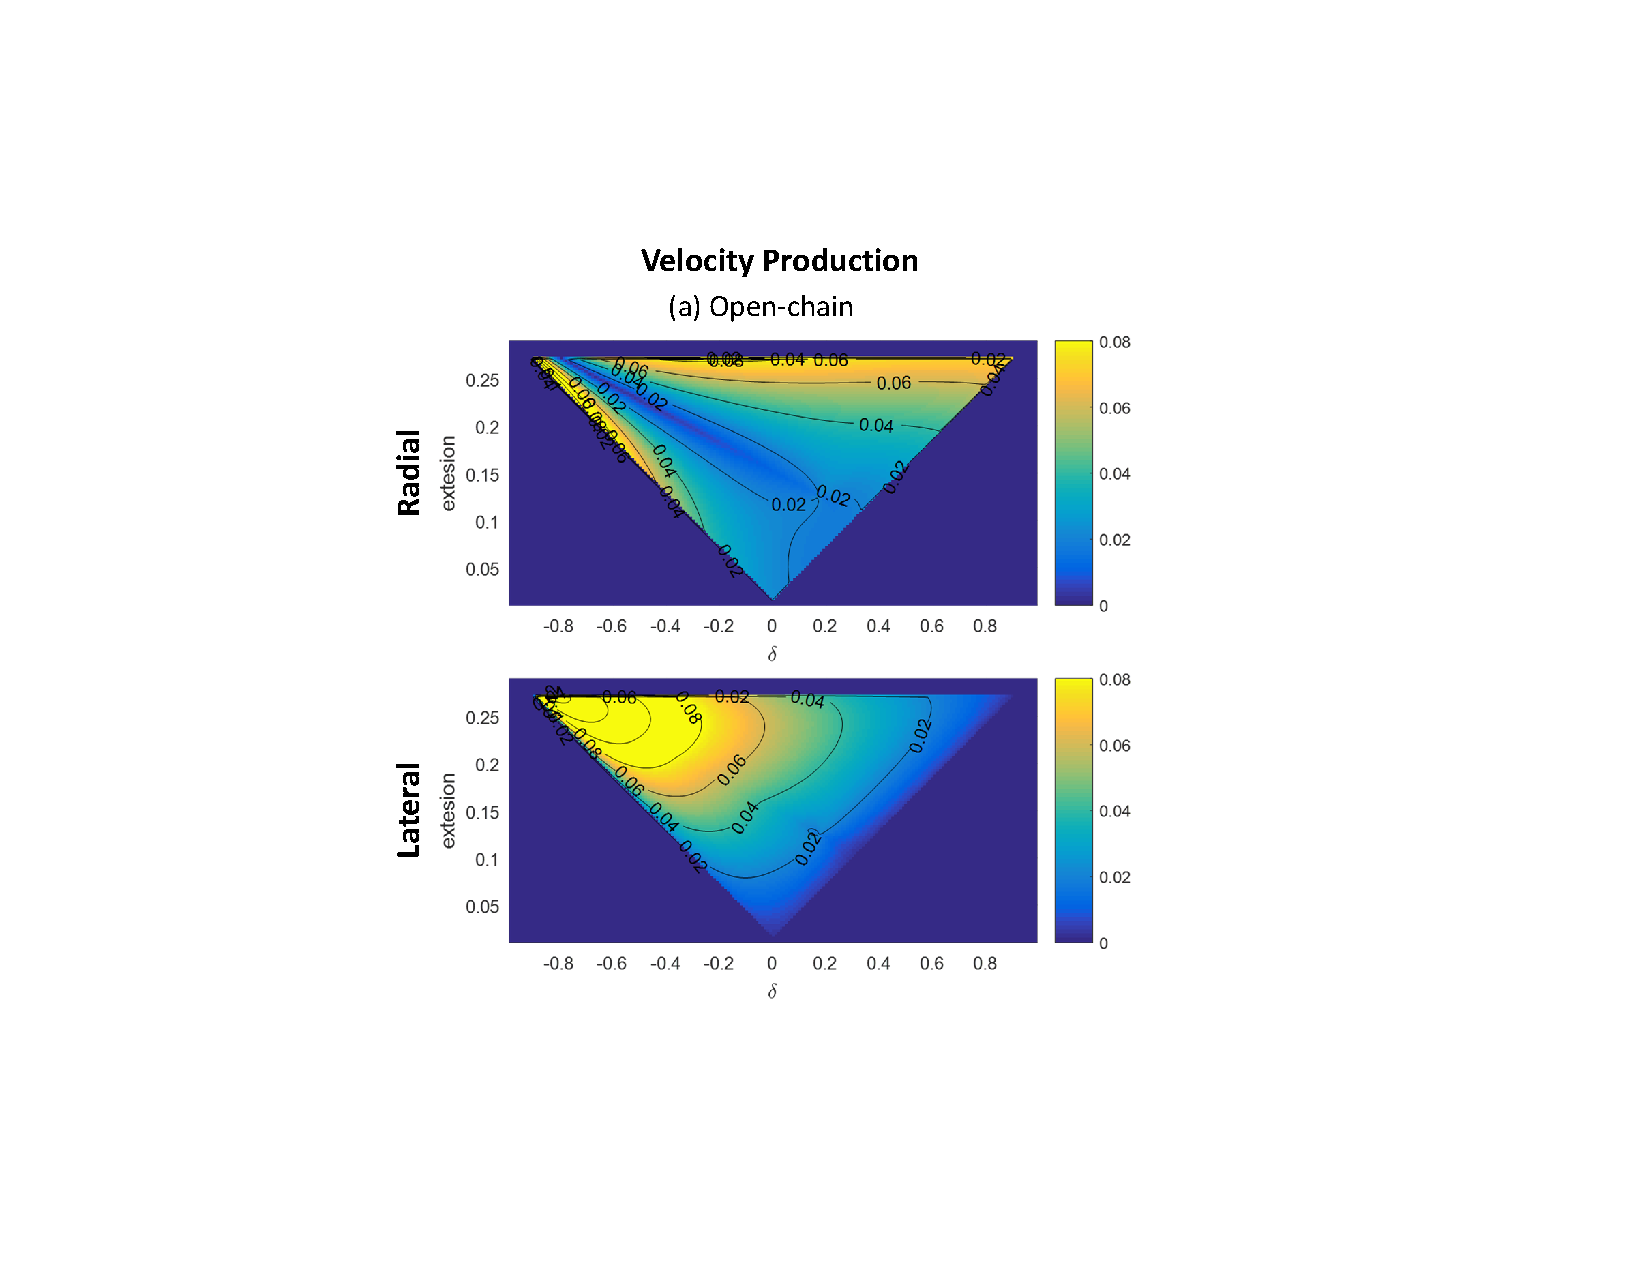
\includegraphics{vel_openChain.pdf}}
		\caption{Velocity production in radial and lateral directions for open chain design}
		\label{fig:vel_openChain}
	\end{figure*}
	
	\begin{figure*}
		\centering
		\resizebox{0.7\linewidth}{!}{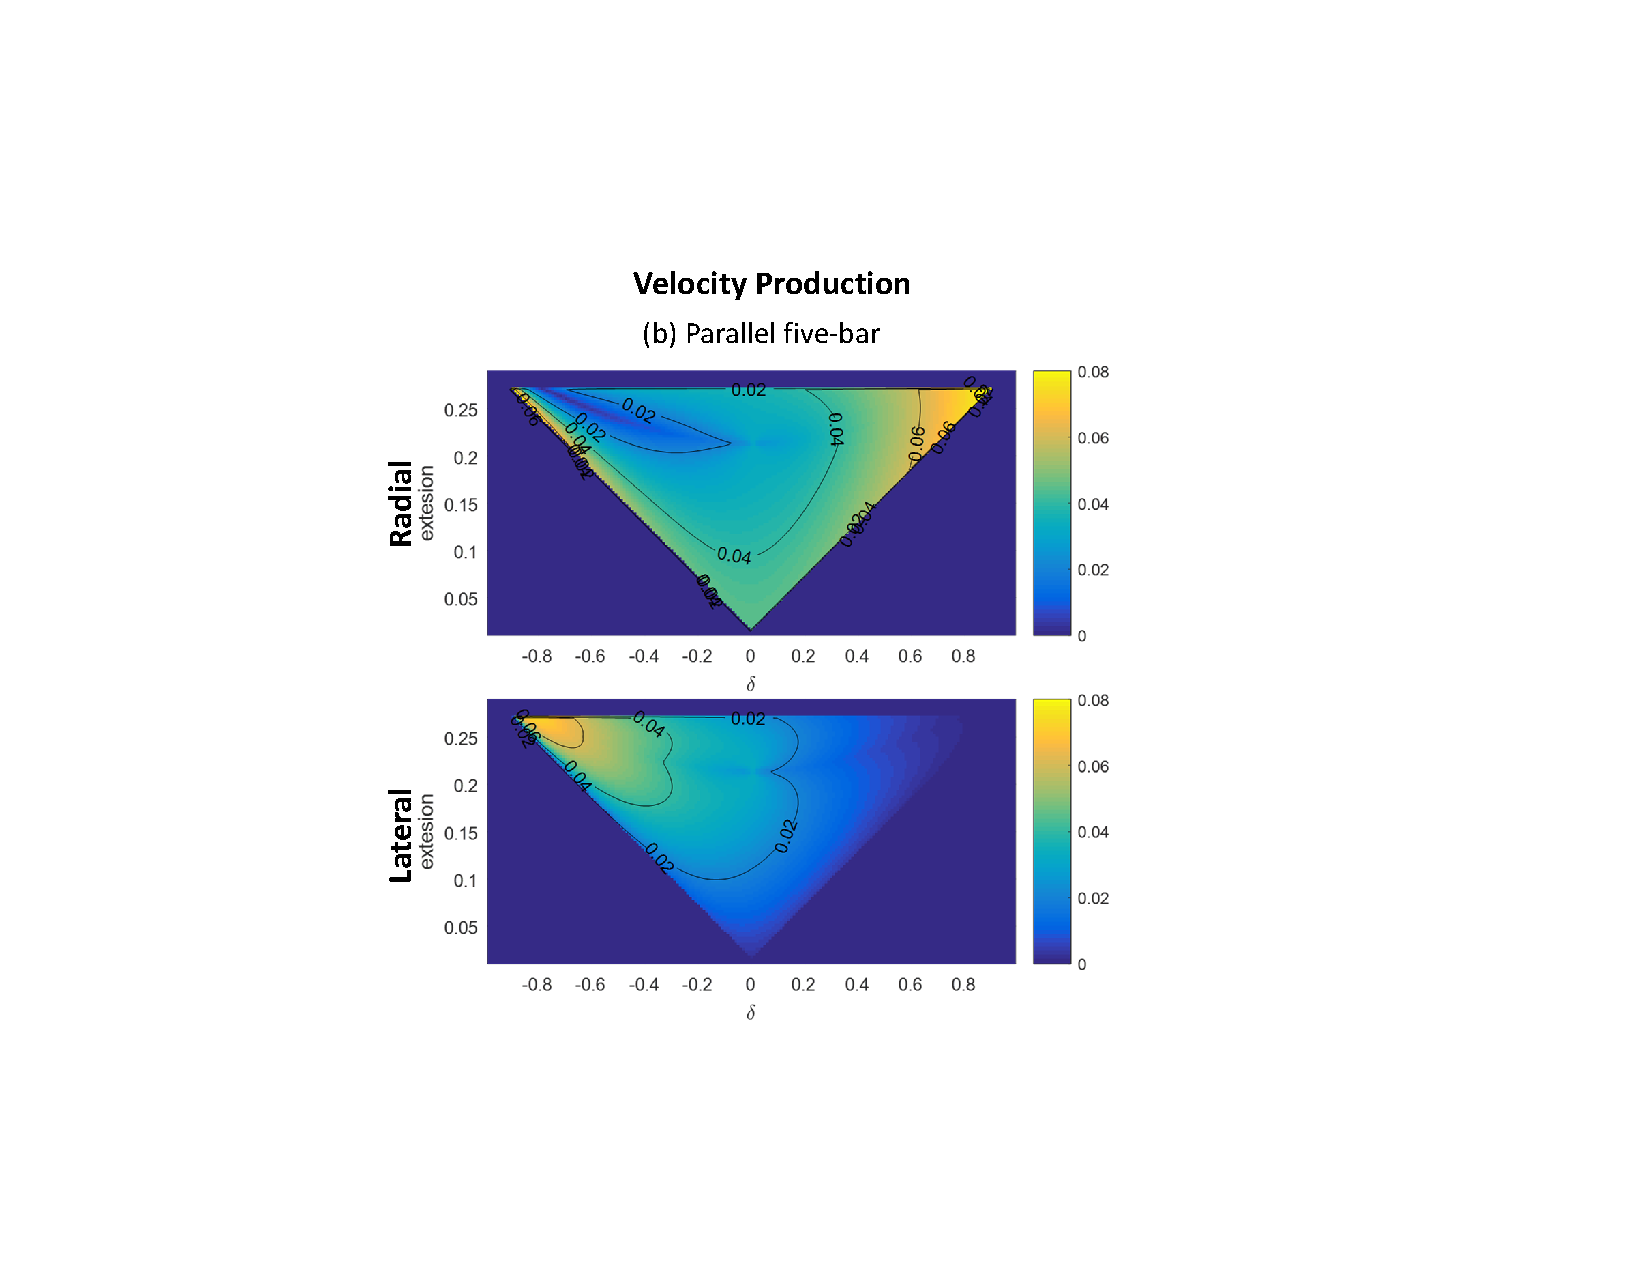
\includegraphics{vel_fiveBar.pdf}}
		\caption{Velocity production in radial and lateral directions for parallel five-bar design}
		\label{fig:vel_fiveBar}
	\end{figure*}
	
	\begin{figure*}
		\centering
		\resizebox{0.7\linewidth}{!}{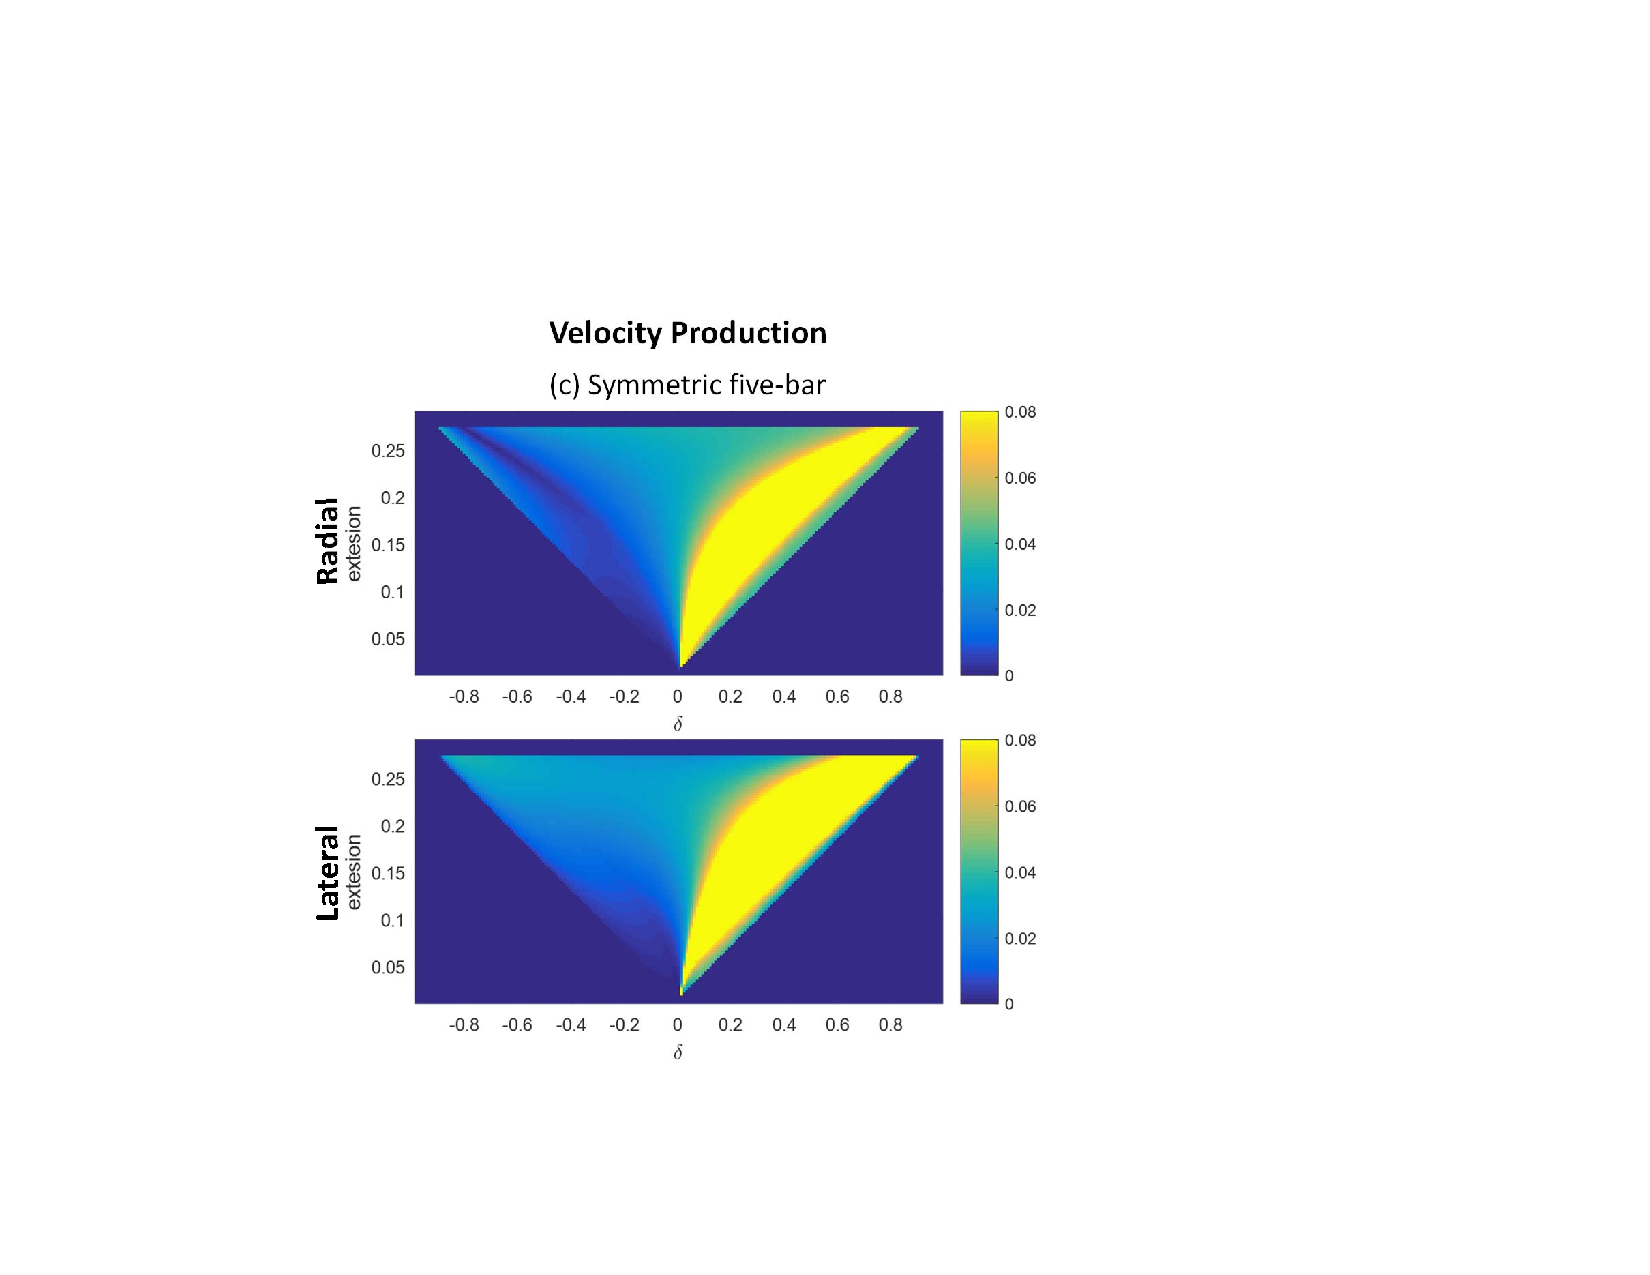
\includegraphics{vel_symm.pdf}}
		\caption{Velocity production in radial and lateral directions for symmetric five-bar design}
		\label{fig:vel_symm}
	\end{figure*}

	Velocity production ellipsoid characterizes how unit joint velocity from motors will reflect as end-effector velocity. Solution to equation \ref{eq:vel_production} forms the velocity production ellipsoid. The major and minor axes of the velocity production ellipsoid represent the end-effector's strongest and weakest ability to produce velocity at the respective directions.
	
	\begin{equation}\label{eq:vel_production}
		E_{velocity} := \{V | (J^{-1}v)^T(J^{-1}v)=||\omega|| , ||\omega||=1\}
	\end{equation}
	
	Radial/Lateral velocity production is defined as the end-effector velocity in radial/lateral directions given unit joint angular velocity input. Figure \ref{fig:force_openChain} \ref{fig:force_fiveBar} \ref{fig:force_symm} show how velocity production ability changes over $extension$ and $\delta$.


%-------------------------------------------
% ----------Proprioceptive Sensing----------
\subsection{Proprioceptive Sensing}
\label{sec:propSense}

	Proprioceptive sensitivity ellipsoid represents how unit force applied at the end-effector is visible to the motors. Solution to equation	 \ref{eq:sensitivity} forms the proprioceptive sensitivity ellipsoid.

	\begin{equation}\label{eq:sensitivity}
		E_{sensitivity} := \{\tau | \tau^T J^{-1}J^{-T}\tau = ||F||, ||F||=1\}
	\end{equation}
	
	\begin{figure*}
		\centering
		\resizebox{\linewidth}{!}{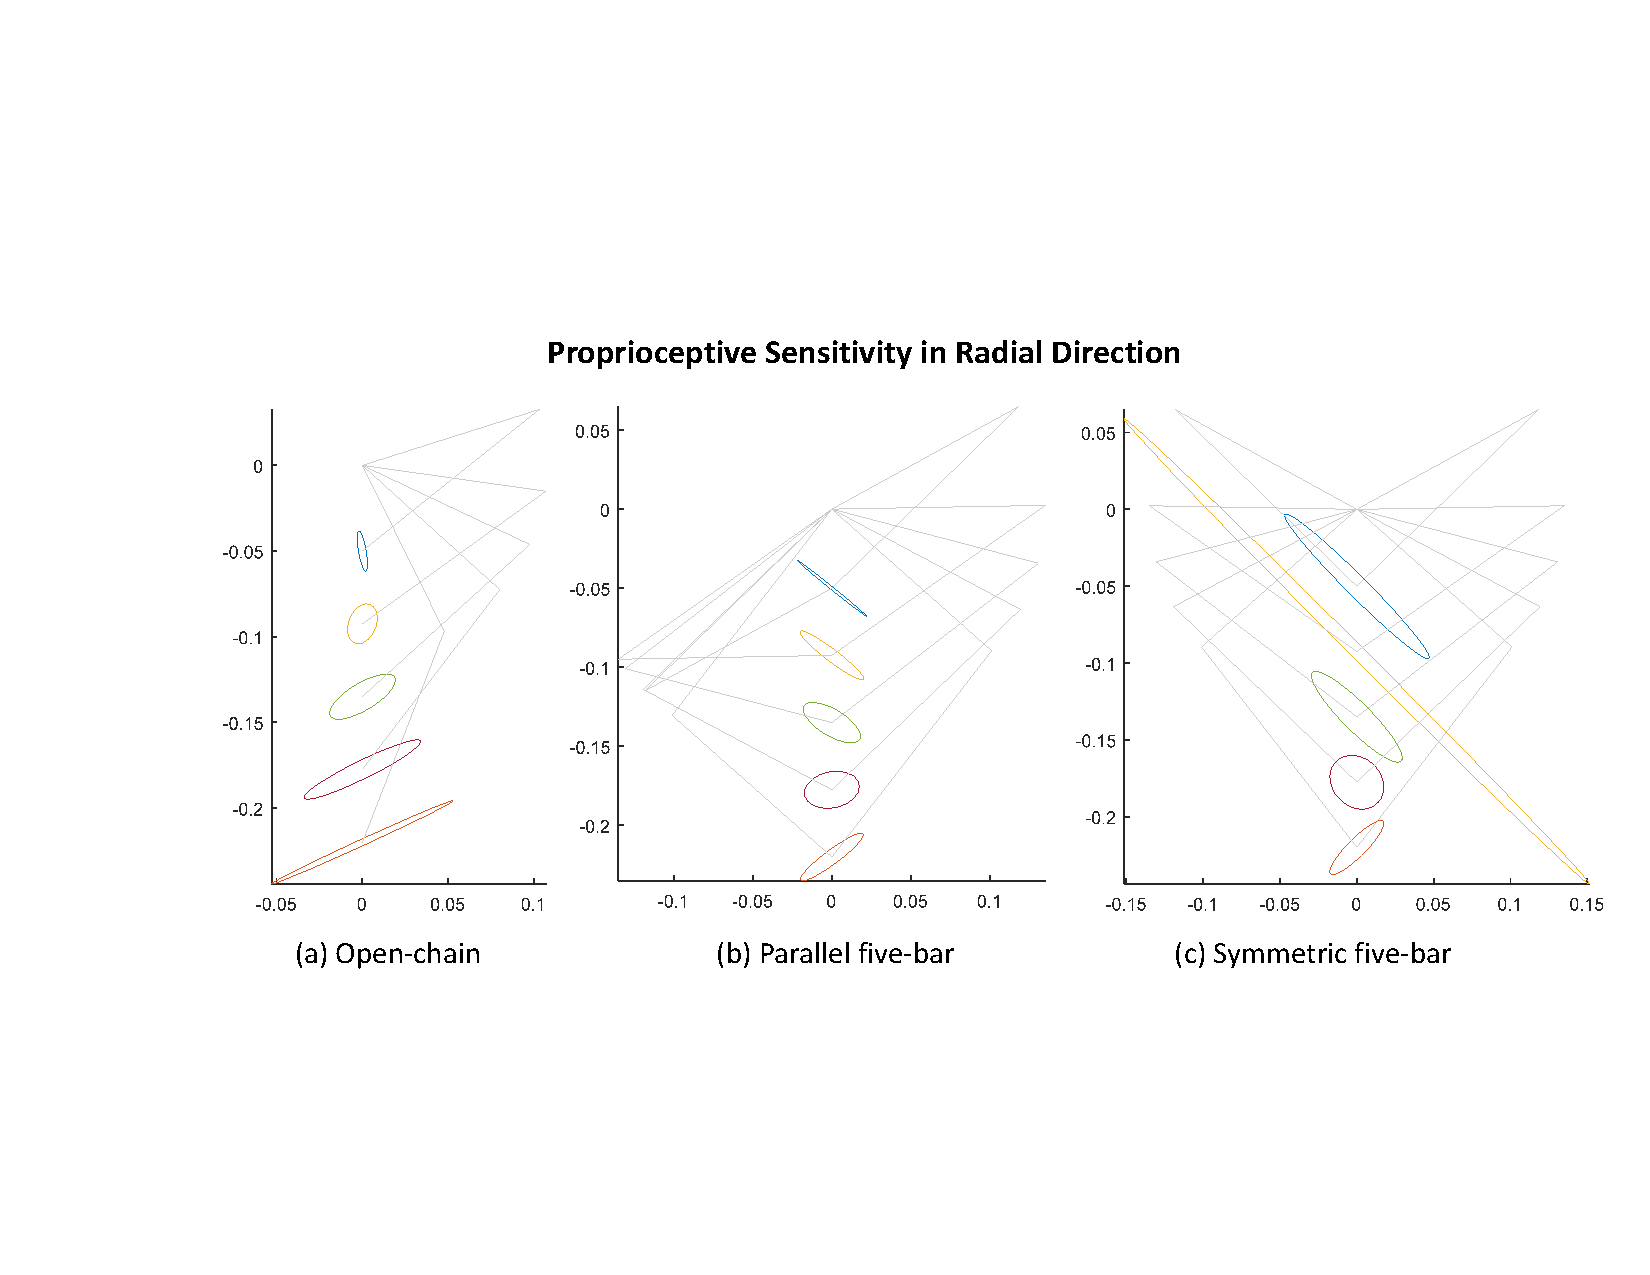
\includegraphics{egLink_sensi_Ellip.pdf}}
		\caption{Proprioceptive Sensitivity in radial direction for an example linkage design of Open-chain, Parallel five-bar and Symmetric five-bar}
		\label{fig:egLink_sensi_Ellip}
	\end{figure*}
	
	\begin{figure*}
		\centering
		\resizebox{0.7\linewidth}{!}{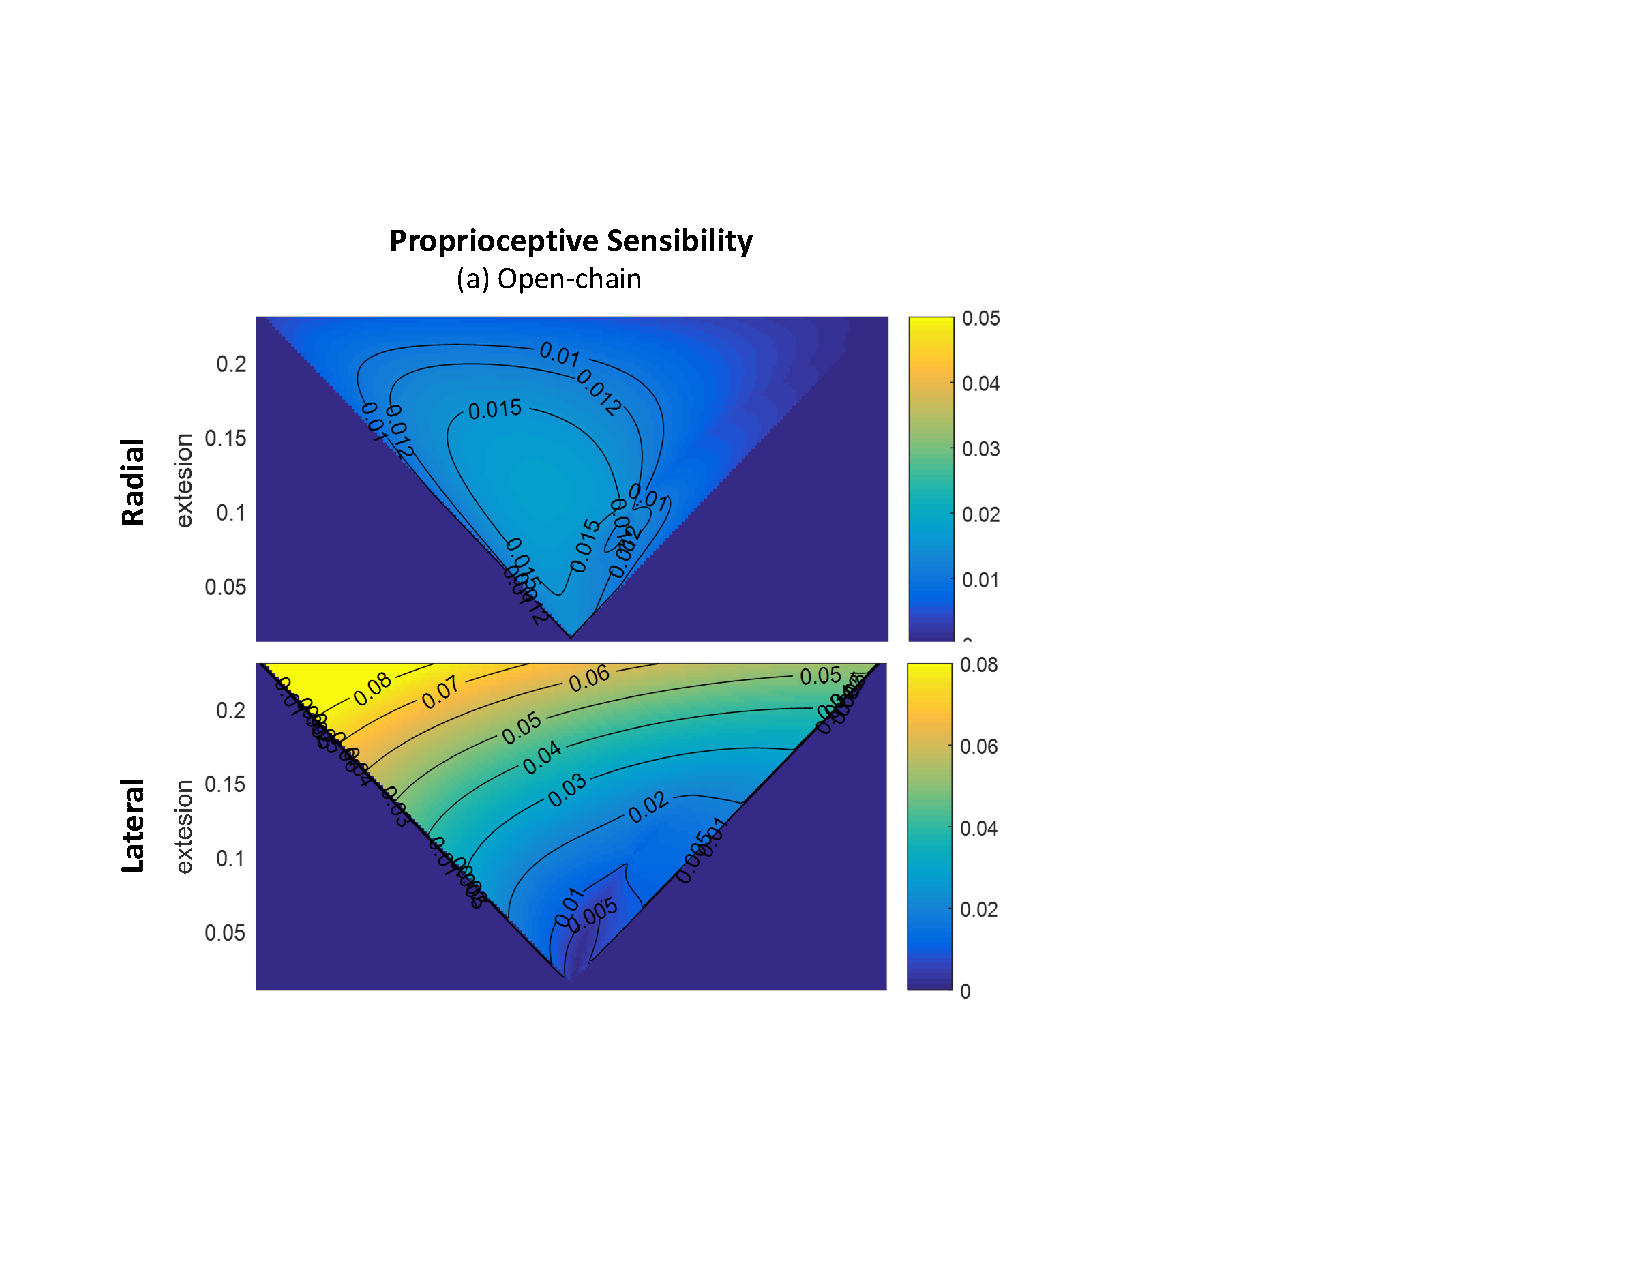
\includegraphics{sensitivity_openChain.pdf}}
		\caption{Proprioceptive Sensitivity in radial and lateral directions for the open-chain design}
		\label{fig:pro_sensitivity_openChain}
	\end{figure*}
	
	\begin{figure*}
		\centering
		\resizebox{0.7\linewidth}{!}{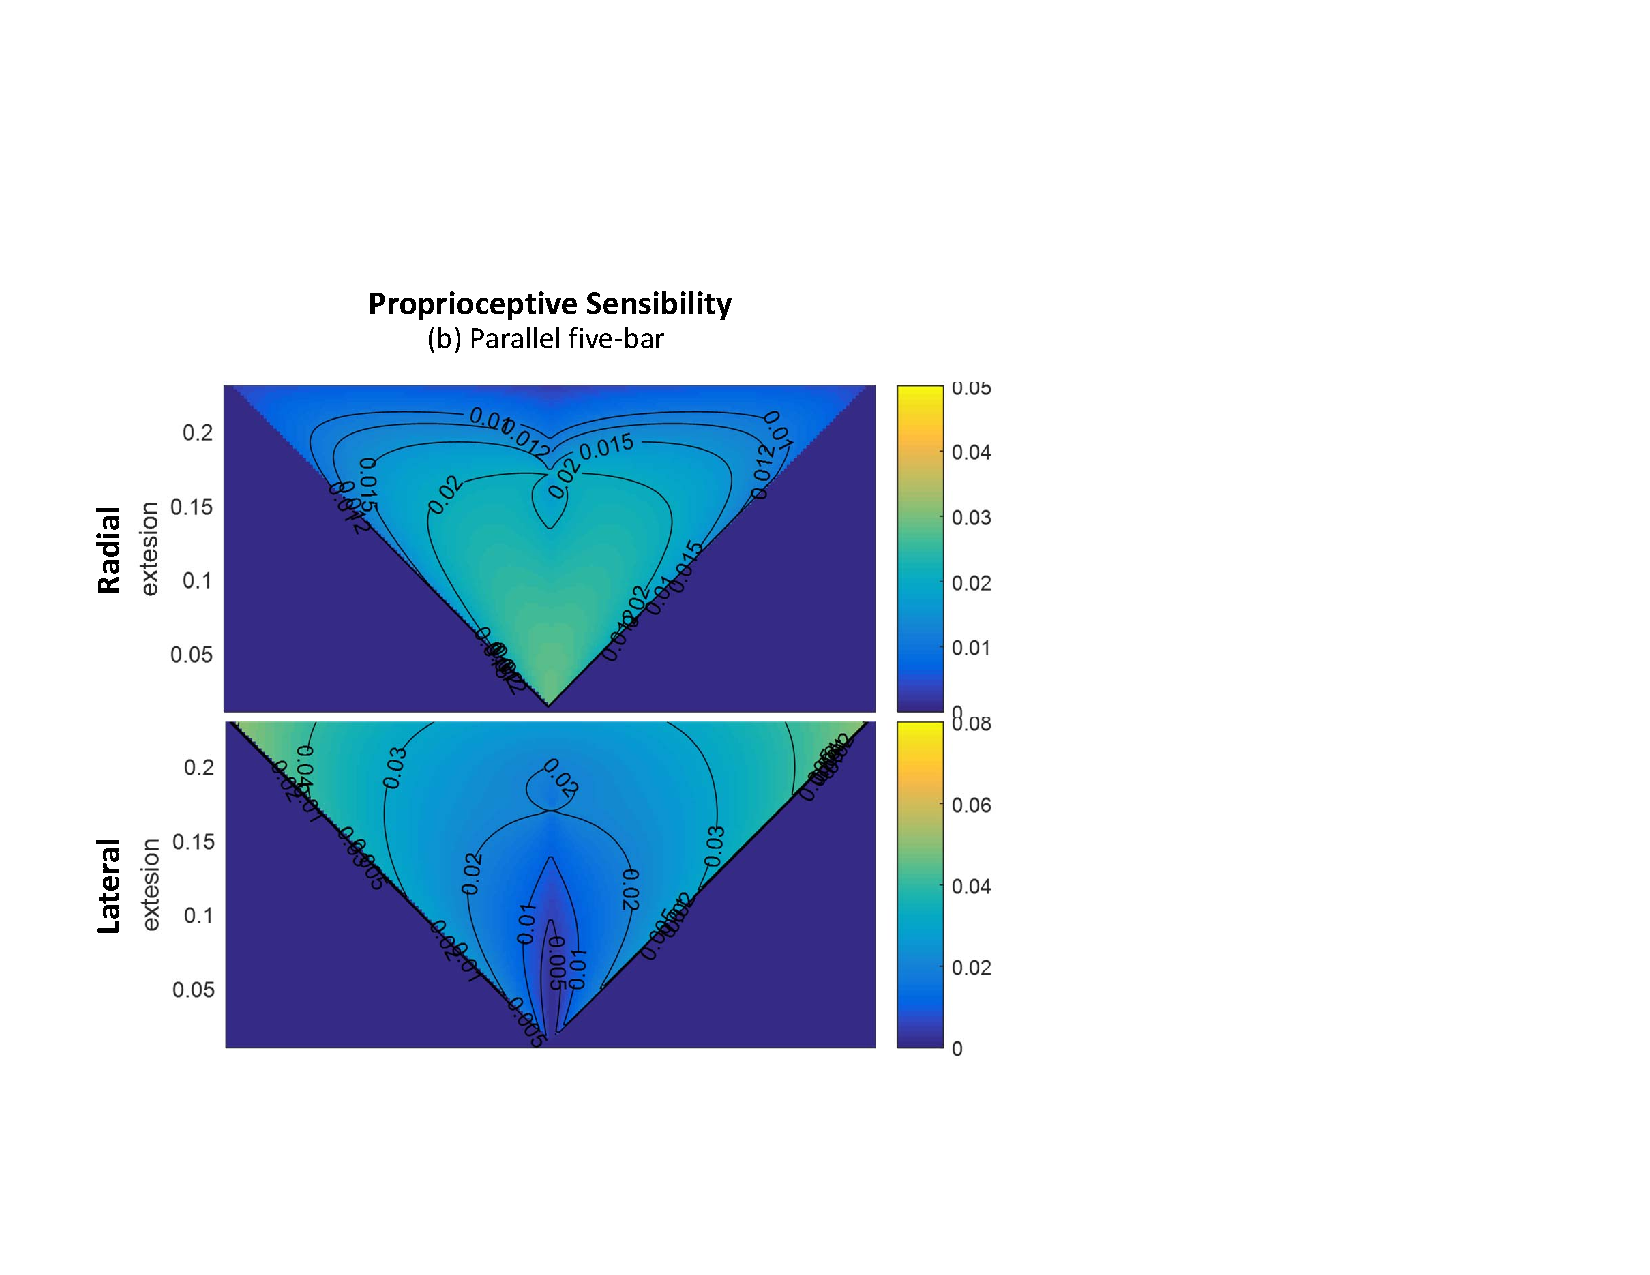
\includegraphics{sensitivity_fiveBar.pdf}}
		\caption{Proprioceptive Sensitivity in radial and lateral directions for the parallel five-bar design}
		\label{fig:pro_sensitivity_fiveBar}
	\end{figure*}
	
	\begin{figure*}
		\centering
		\resizebox{0.7\linewidth}{!}{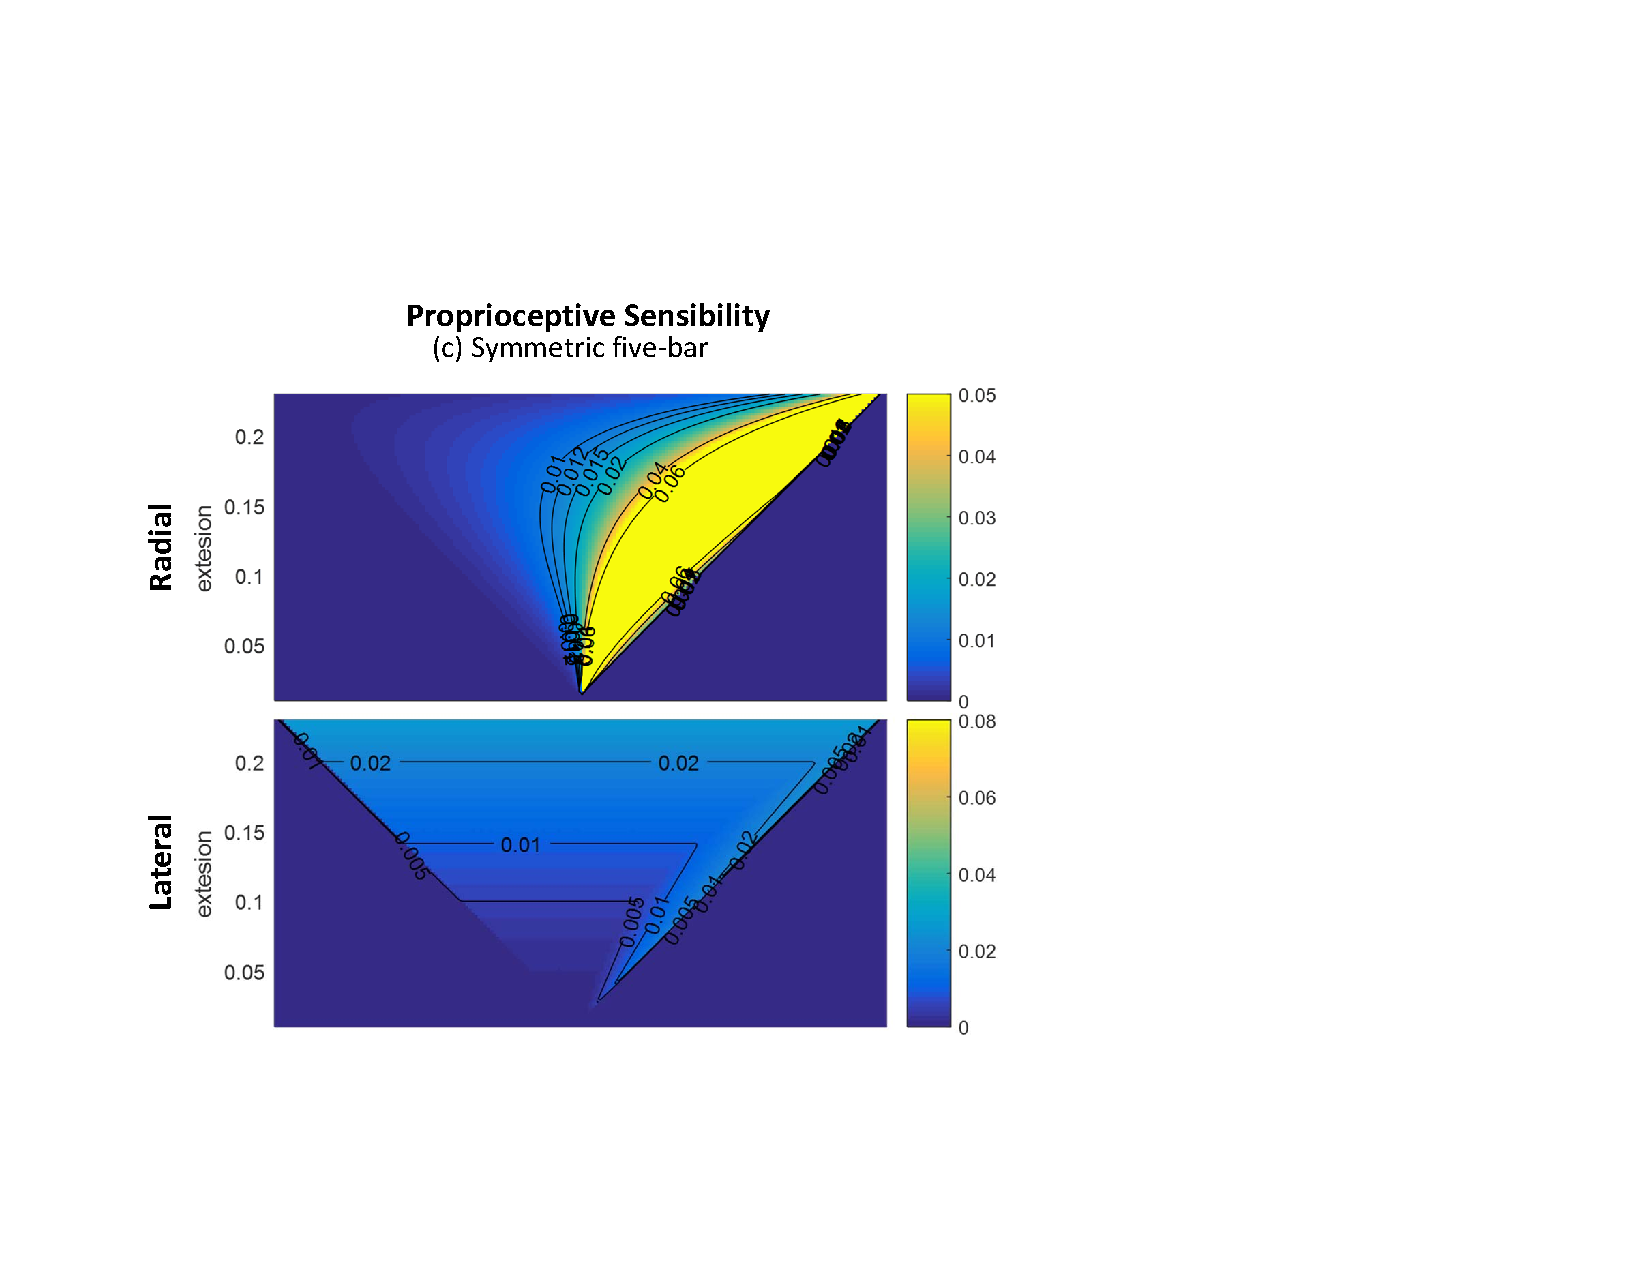
\includegraphics{sensitivity_symm.pdf}}
		\caption{Proprioceptive Sensitivity in radial and lateral directions for the symmetric five-bar design}
		\label{fig:pro_sensitivity_symm}
	\end{figure*}
	
	An example linkage design for the thee leg topologies is shown in Figure \ref{fig:egLink_sensi_Ellip} where design parameter $\delta$ is fixed as 0.1 and workspace parameter $extension$ is varied. The figure shows that in this specific example, the area enclosed by proprioceptive sensitivity ellipsoid is almost the same with symmetric five-bar slightly better.

	It is worth remarking that similar to force and velocity production, proprioceptive sensitivity should not only be considered in the radial direction, but also in the lateral direction. Radial/Lateral Proprioceptive Sensitivity is defined as the joint torque magnitude when radial/lateral unit force is applied at the end-effector. Figure \ref{fig:pro_sensitivity_openChain}, \ref{fig:pro_sensitivity_fiveBar}, \ref{fig:pro_sensitivity_symm} show how proprioceptive sensitivity changes over design parameters $extension$ and workspace variable $\delta$.
	
	Figure \ref{fig:pro_sensitivity_openChain}, \ref{fig:pro_sensitivity_fiveBar}, \ref{fig:pro_sensitivity_symm} show that while symmetric five-bar has excellent radial proprioceptive sensitivity, its lateral sensitivity is relatively poorer. In contrast, Open-chain design has better lateral proprioceptive sensitivity. Higher lateral sensitivity renders open-chain design advantageous in controlling horizontal forces, which is useful in applications such as jumping forward to precise location, control horizontal speed in running and so on.
	
	%-------------------------------------------
	% ----------Power Delivery----------
	\subsection{Power Delivery}
	\label{sec:powerDelivery}
	
	Since the velocity and force ellipsoids have their major axis coincide with the other's minor axis and vice versa, this means they are conjugate of each other. Thus the power delivery in every direction of the linkage design is assumed to be the same. But the manipulator analysis is static so only fixed instances are considered.
	
	
	%-------------------------------------------
	% ----------Linkage Design----------
	\subsection{Linkage Design}
	\label{sec:LinkageDesign}
	
	Although symmetric five-bar has excellent velocity production ability in both radial and lateral directions, its proprioceptive sensitivity in lateral direction is not very good. In addition, both parallel and symmetric five-bar design suffer from too large sweep volume, which is not desirable for quadrupedal robot locomotion, especially in unstructured terrain. Therefore, open-chain topology is chosen to be the linkage design.
	
	The previous sections have provided a recipe to come up with suitable link design for specific applications. An optimal design could be found by defining a cost function that pertains to application requirements. 
	
	\begin{equation}\label{eq:obj_func}
		Cost = - (w_{F_r} F_r + w_{F_l} F_l + w_{V_r} V_r + w_{V_l} V_l + w_{S_r} S_r + w_{S_r} S_r) + w_{\delta}\delta
	\end{equation}
	
	
	where $F_r,F_l,V_r,V_l,S_r,S_l$ are the force production and $\delta$ is as defined before, velocity production and proprioceptive sensitivity values in the radial and lateral directions, which is \textbf{normalized} by the average value in the span of $extension$ to get rid of the effect of magnitude of unit. $w_{F_r},w_{F_l},w_{V_r},w_{V_l},w_{S_r},w_{S_r},w_{\delta}$ are weighting factors that corresponds to the values. Higher weight could be put on the value that plays an important role on the application. For example, if a robot is designed to perform mostly in situations where high force production is required while operating in a low velocity region, the weighting factor for force production could be higher and the weighting factors for velocity production could be lower. By the same token, applications where precise force production is required could put higher penalty on the proprioceptive sensitivity term. 
	
	In this application we want to place a balanced emphasis on all the radial and lateral parameters, hence $w_{F_r},w_{F_l},w_{V_r},w_{V_l},w_{S_r},w_{S_r}$ was all set to be equal, and $w_{\delta}$ was set to be 100 times larger than the other weighting factors to prevent optimal point appear at the infeasible region. The final optimized result showed that $\delta$ is very close to zero, which indicates that equal length link is favorable for leg topology.
	
	


\chapter{Hardware Integration}

\section{\textbf{Transmission Design}}
\label{sec:transmissionDesign}

The actuator design philosophy is to make high power actuators with the capability of interacting with the environment. Namely, the actuator should not be stiff as the heavily geared motors, which are widely used in industrial robots. Instead, it should be back-drivable meaning that the torque applied at the output shaft should be felt at the input shaft. The benefits are threefold, firstly, back-drivability prevents geatboxes from being damaged by external forces; second, it allows for proprioceptive sensing\cite{Seok2012}; thirdly, allows for fast dynamics in legged locomotion.

After the motor selection and gear ratio is determined from previous sections, focus was put on how to design the transmission system so that it can achieve the desired gear ratio while satisfying dimensional constraints.

\subsection{\textbf{Transmission Design Comparison}}
\label{sec:transmissionComparison}

\textbf{Harmonic drive} is composed of the wave generator, flexspline and circular spline. It could provide high gear ratio typically between 30:1 to 200:1 with zero backlash. Harmonic drive is employed by the quadrupedal robot starlETH\cite{Hutter2013} and the bipedal robot ATRIAS\cite{Hubicki2016}. However, harmonic drive is not back-drivable, which contradicts with our design paradigm.

\textbf{Cycloidal gearbox} has very low backlash and high torsional stiffness. It can operate quietly and withstand shock load. Bipedal robot Cassie uses cycloidal gearbox as the transmission. The drawback of cycloidal gearbox is that it requires customizing high precision parts.

\textbf{Single stage planetary gearbox} has high efficiency and the load could be distributed between planet gears, and standard gears are widely available at low cost. Nevertheless, no gear combination could provide the desired gear ratio for the given dimensional limitation with pitch of 0.4.

\textbf{Compound planetary gearboxes} have the benefits of single stage planetary gearboxes while providing more compact design for there are two stages for the planet gear. There are a range of gear teeth selection for the given dimensional limits. It is adopted as the transmission system design considering the dimensional limit and gear ratio requirement of the motor design.

\subsection{\textbf{Compound Planetary Gearbox Design}}
\label{sec:compoundGearBox}

\begin{figure}
	\centering
	\resizebox{1.0\linewidth}{!}{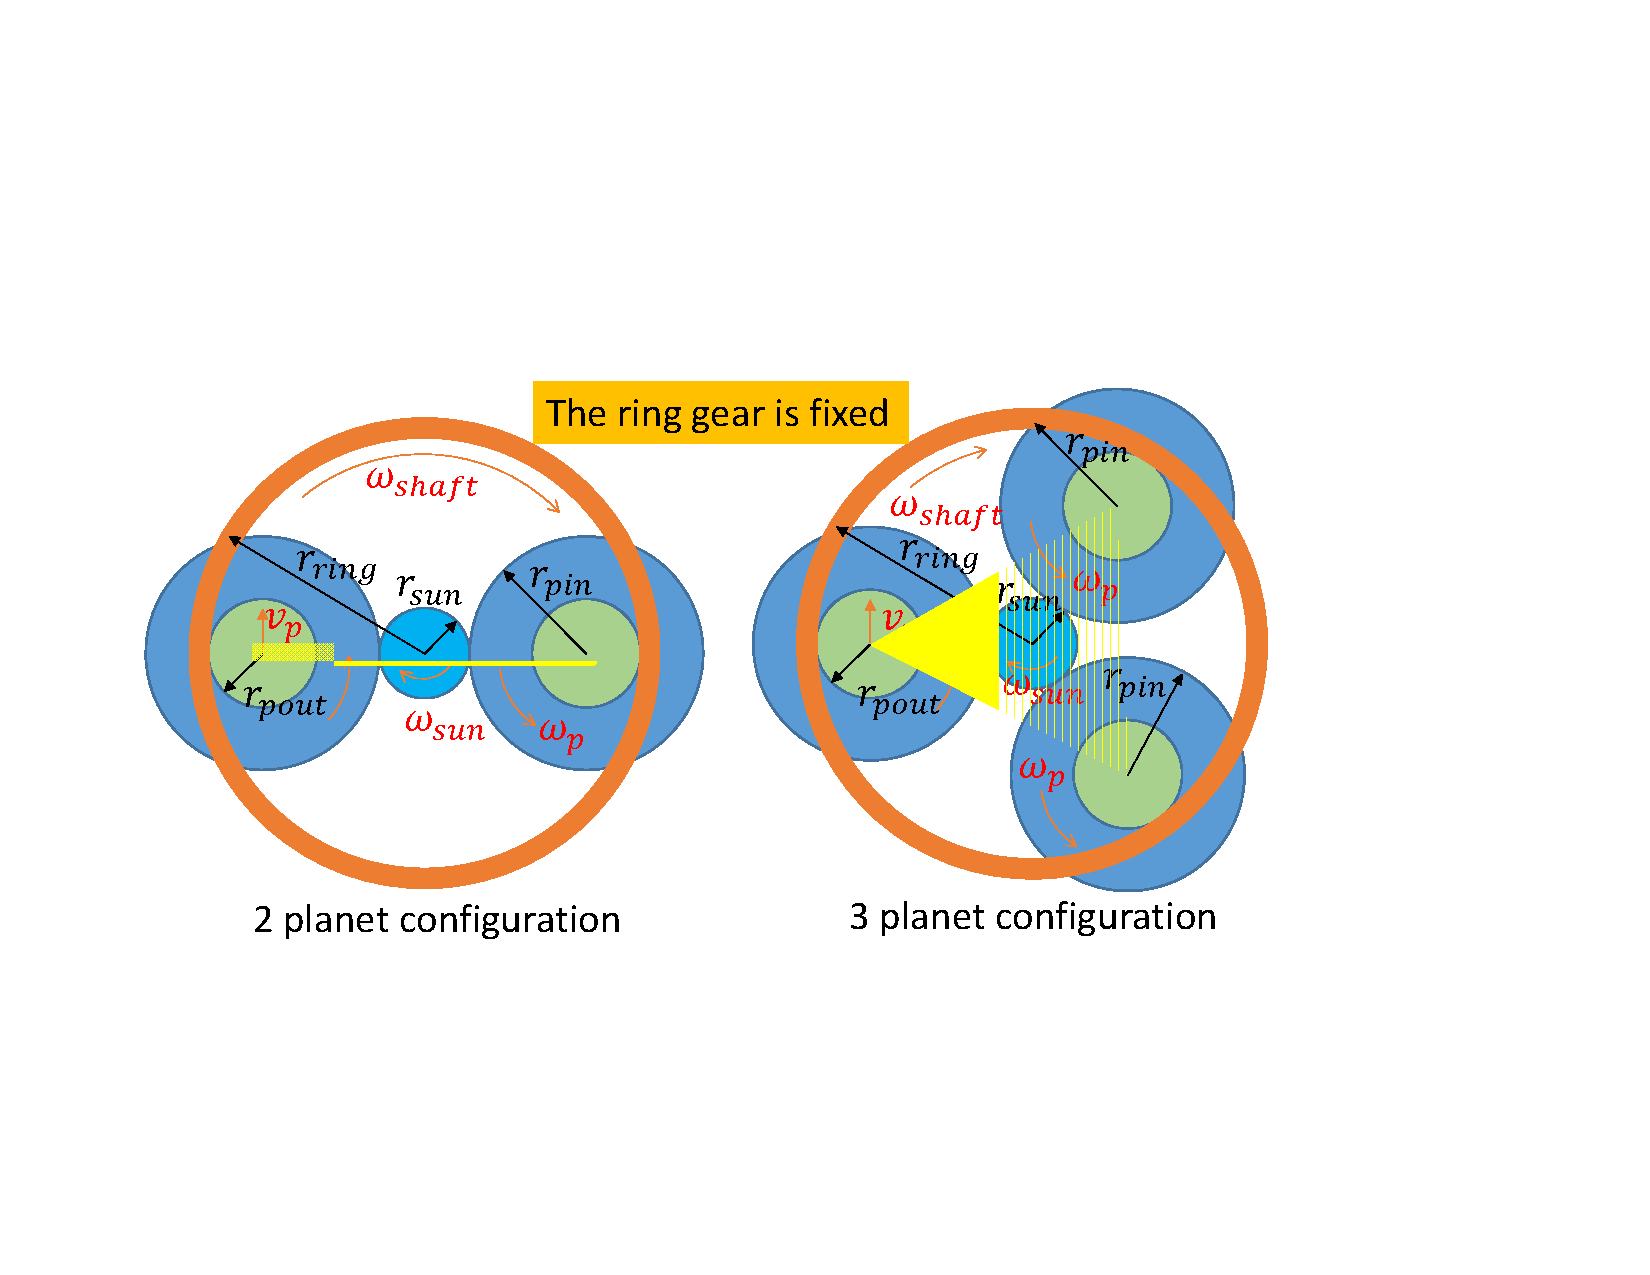
\includegraphics{planetaryGearbox.pdf}}
	\caption{Schematics of Compound Planetary Gearbox Configurations. (left) 2 planet configuration, (right) 3 planet configuration}
	\label{fig:planetaryGearbox}
\end{figure}

The objective of compound planetary gearbox design is to achieve desired gear ratio within dimensional constraints imposed by motor selection. In order to derive the gear ratio for given gear teeth number, a schematics of the two-stage compound planetary gearbox is used as shown in Figure \ref{fig:planetaryGearbox}. For given gear teeth numbers, both configurations in Figure \ref{fig:planetaryGearbox} are equivalent. Some assumptions for this analysis is posed here: 

\begin{enumerate}
	\item The sun gear located at the center is the input.
	\item The output shaft shown as yellow transparent shape is the output.
	\item The output shaft is connected to the axes of all the planet gears.
	\item The sun gear is meshed with input planet gears.
	\item The ring gear is meshed with output planet gears.
	\item The ring gear is fixed.
\end{enumerate}

Velocity equivalence is used to calculate the gear ratio.
\begin{eqnarray}
\omega_{sun} r_{sun} =& v_p + \omega_p r_{pin}\\
v_p =& \omega_{p} r_{pout}\\
\omega_p =& \frac{\omega_{sun}r_{sun}}{r_{pout}+r_{pin}}\\
\omega_{shaft} =& \frac{\omega_{p}r_{pout}}{r_{sun}+r_{pin}}
\end{eqnarray}
where $\omega_{shaft}$ is the angular velocity of the output shaft and the rest of the variable definitions could be found in Table \ref{tab:varDefGearbox}.

Therefore, the gear ratio of a compound planetary gearbox could be formulated as:
\begin{equation}
GR = \frac{\omega_{sun}}{\omega_{shaft}} = \frac{(r_{pout}+r_{pin})(r_{sun}+r_{pin})}{r_{sun}r_{pout}} = \frac{(N_{pout}+N_{pin})(N_{sun}+N_{pin})}{N_{sun}N_{pout}}
\end{equation}

\begin{table}[bp]
	\centering
	\caption{Variable Definition for Gear Ratio Calculation}
	\begin{tabular}{lcccc}\hline\hline
		& Sun gear		& Input planet	& Output planet	& Ring gear \\ \hline
		Pitch diameter	& $r_{sun}$	   	& $r_{pin}$		& $r_{pout}$	& $r_{ring}$\\
		Angular velocity& $\omega_{sun}$& $\omega_{p}$	& $\omega_{p}$	& N/A		\\
		Linear velocity	& N/A			& $v_p$			& $v_p$			& N/A		\\
		Teeth number	& $N_{sun}$		& $N_{pout}$	& $N_{pout}$	& $N_{ring}$\\ \hline
	\end{tabular}
	\label{tab:varDefGearbox}
\end{table}

The planetary gearbox shown in Figure \ref{fig:gearbox} utilizes two-stage compound planet gears to provide desired gear ratio while satisfying the dimensional constraints imposed by motor selection. 

The constraints for choosing teeth numbers are listed as follows:

\begin{enumerate}
	\item The teeth number of sun gear ($N_{sun}$) and ring gear ($N_{ring}$) could both be divided by the number of planet gears.
	\item The pitch circles of sun gear and planet gears, as well as that of planet gears and the ring gear should be externally tangent, 
	
	i.e. $r_{ring}=r_{sun}+r_{pin}+r_{pout}$ or $N_{ring}=N_{sun}+N_{pin}+N_{pout}$.
	\item The gear ratio $GR$ should be within the range of 22 - 25.
	\item The radius of the gearbox should be less than 25 mm, 
	
	i.e. $Max[r_{ring},r_{sun}+2r_{pin}]<12.5 mm$
	\item The teeth number for sun gear $N_{sun}$ should be no less than 6. Other wise the meshing would be problematic because the profile of gear teeth would be distorted too much.
\end{enumerate}

On top of the constraints, some practical issues were also considered in choosing gear teeth. Ideally, the phase difference between two stages of the planet gears should be the same. However, in compound gear manufacturing, the phase differnce could not be well maintained. To solve this problem, the planet gear teeth combination was chosen to be 16/53, which only share the common factor of 1. This choice provides tunable backlash with $2.1^{\circ}$ increment in the gearbox assembly. This is very similar to the working principle of a mechanical caliper, which uses two scales (main scale and vernier scale) with small difference to achieve high precision.

A large number of teeth combinations were enumerated taking into account all the constraints. The optimal gear teeth choice emerged as $N_{sun} = 12; N_{pin} = 53; N_{pout} = 16; N_{ring} = 81$ and the gear ratio is 23.3594.

All gears are custom made by \textit{HPC Gears Ltd} with 0.4 pitch and pressure angle of $20^{\circ}$.



\section{\textbf{Mechanical Design of The Leg}}
\label{sec:LegDesign}

With actuator from $\color{red}section$ and linkage design from $\color{red}section$, this section presents a detailed mechanical design layout of the leg. The leg module is composed of three motor modules(HIP/KNEE/ABAD), each has a motor coil and a planetary gearbox with moderate gear ratio to achieve the Quasi-Direct-Drive\cite{20162016} strategy. To accommodate size limitation imposed by actuator choice, the two-stage compound planetary gearbox is used as the transmission. The leg is design to optimize for large workspace, with the novel HIP-KNEE connection design, the knee joint could rotate $360^{\circ}$, the curved upper link and hollow thigh link design also enables large knee joint workspace.
  
\begin{figure}
	\centering
	\resizebox{1\linewidth}{!}{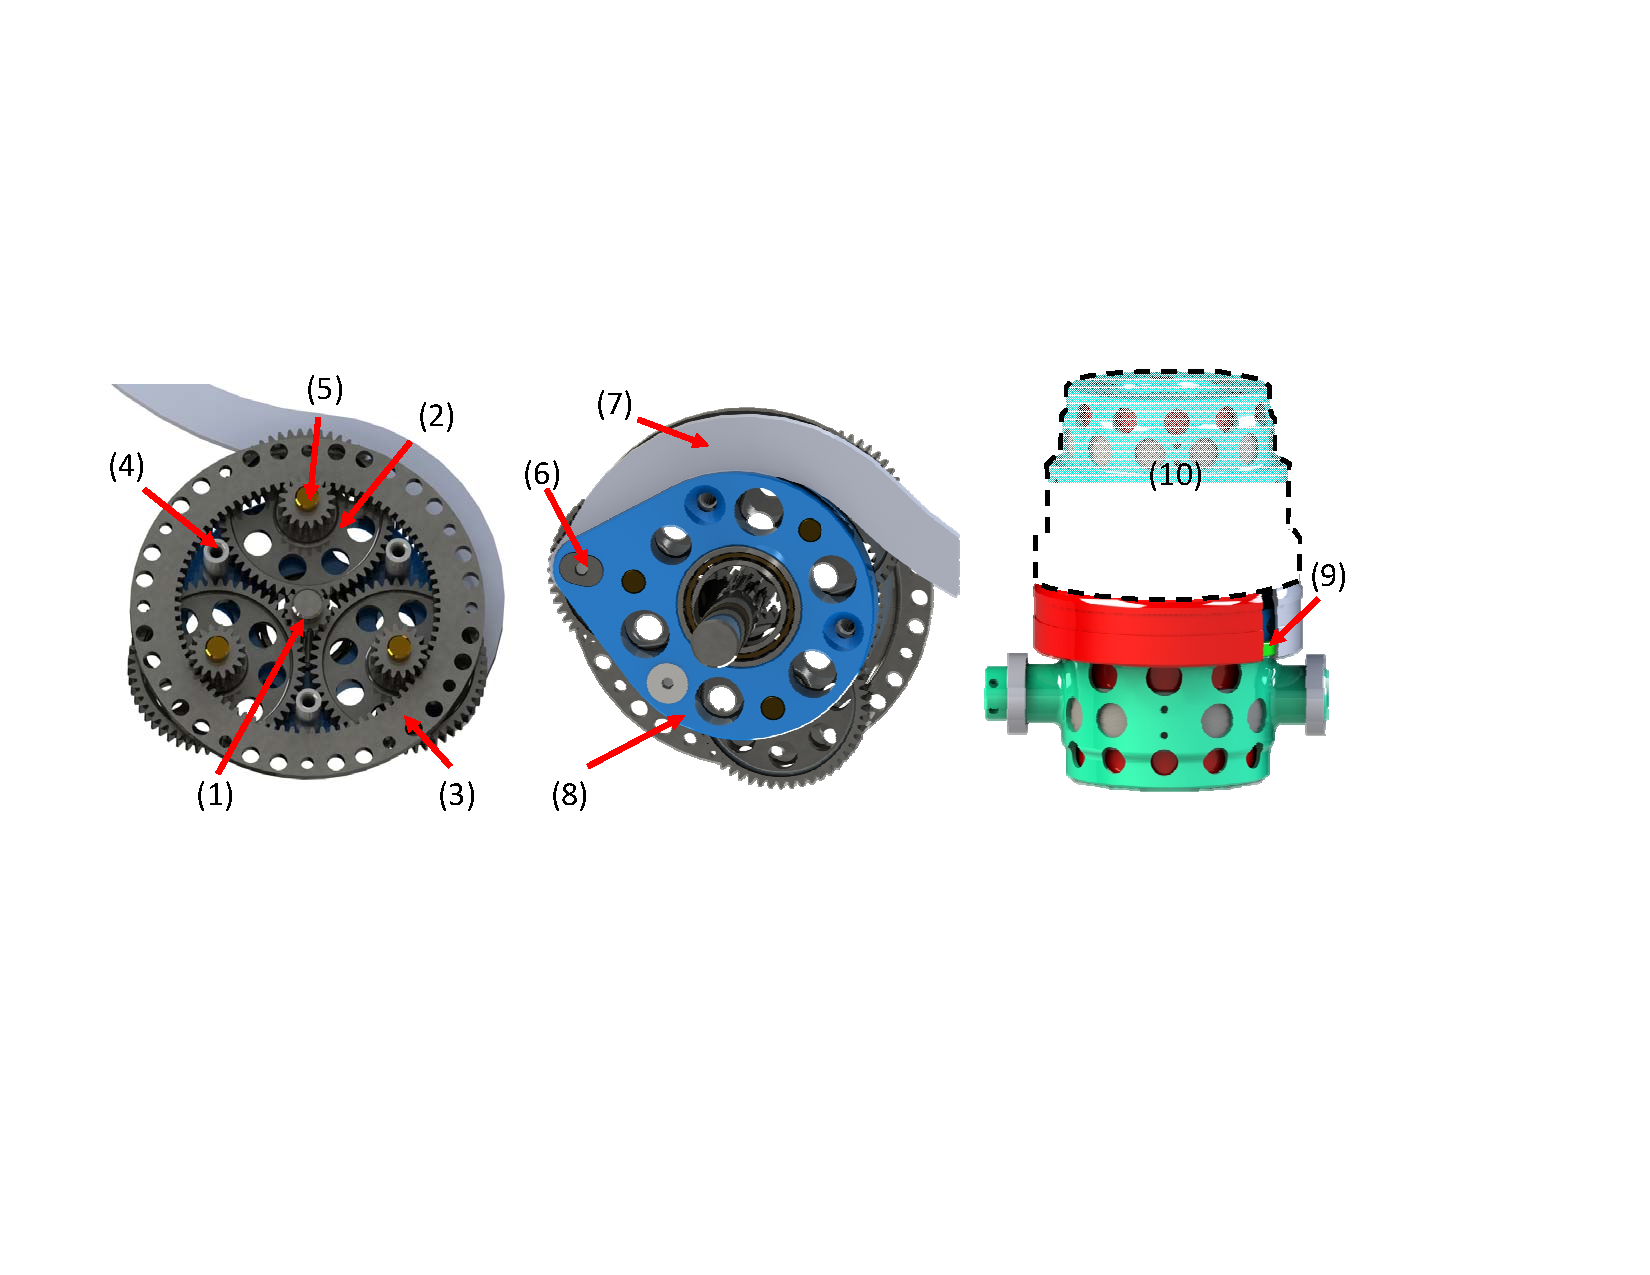
\includegraphics{gearbox.pdf}}
	\caption{Planetary gearbox design with three compound planet gears (left); curved upper-link design (middle); hip and knee motor module (right); (1) sun gear, (2) compound planet gear, (3) ring gear, (4) stand-off, (5) brass dowel pin, (6) output pin, (7) upper link, (8) KNEE carrier, (9) KMF PBXS020 bearing, (10) the KNEE motor module}
	\label{fig:gearbox}
\end{figure}



\subsection{\textbf{HIP-KNEE Connection Design}}
\label{sec:Design4ROM}

\begin{figure}
	\centering
	\resizebox{1.0\linewidth}{!}{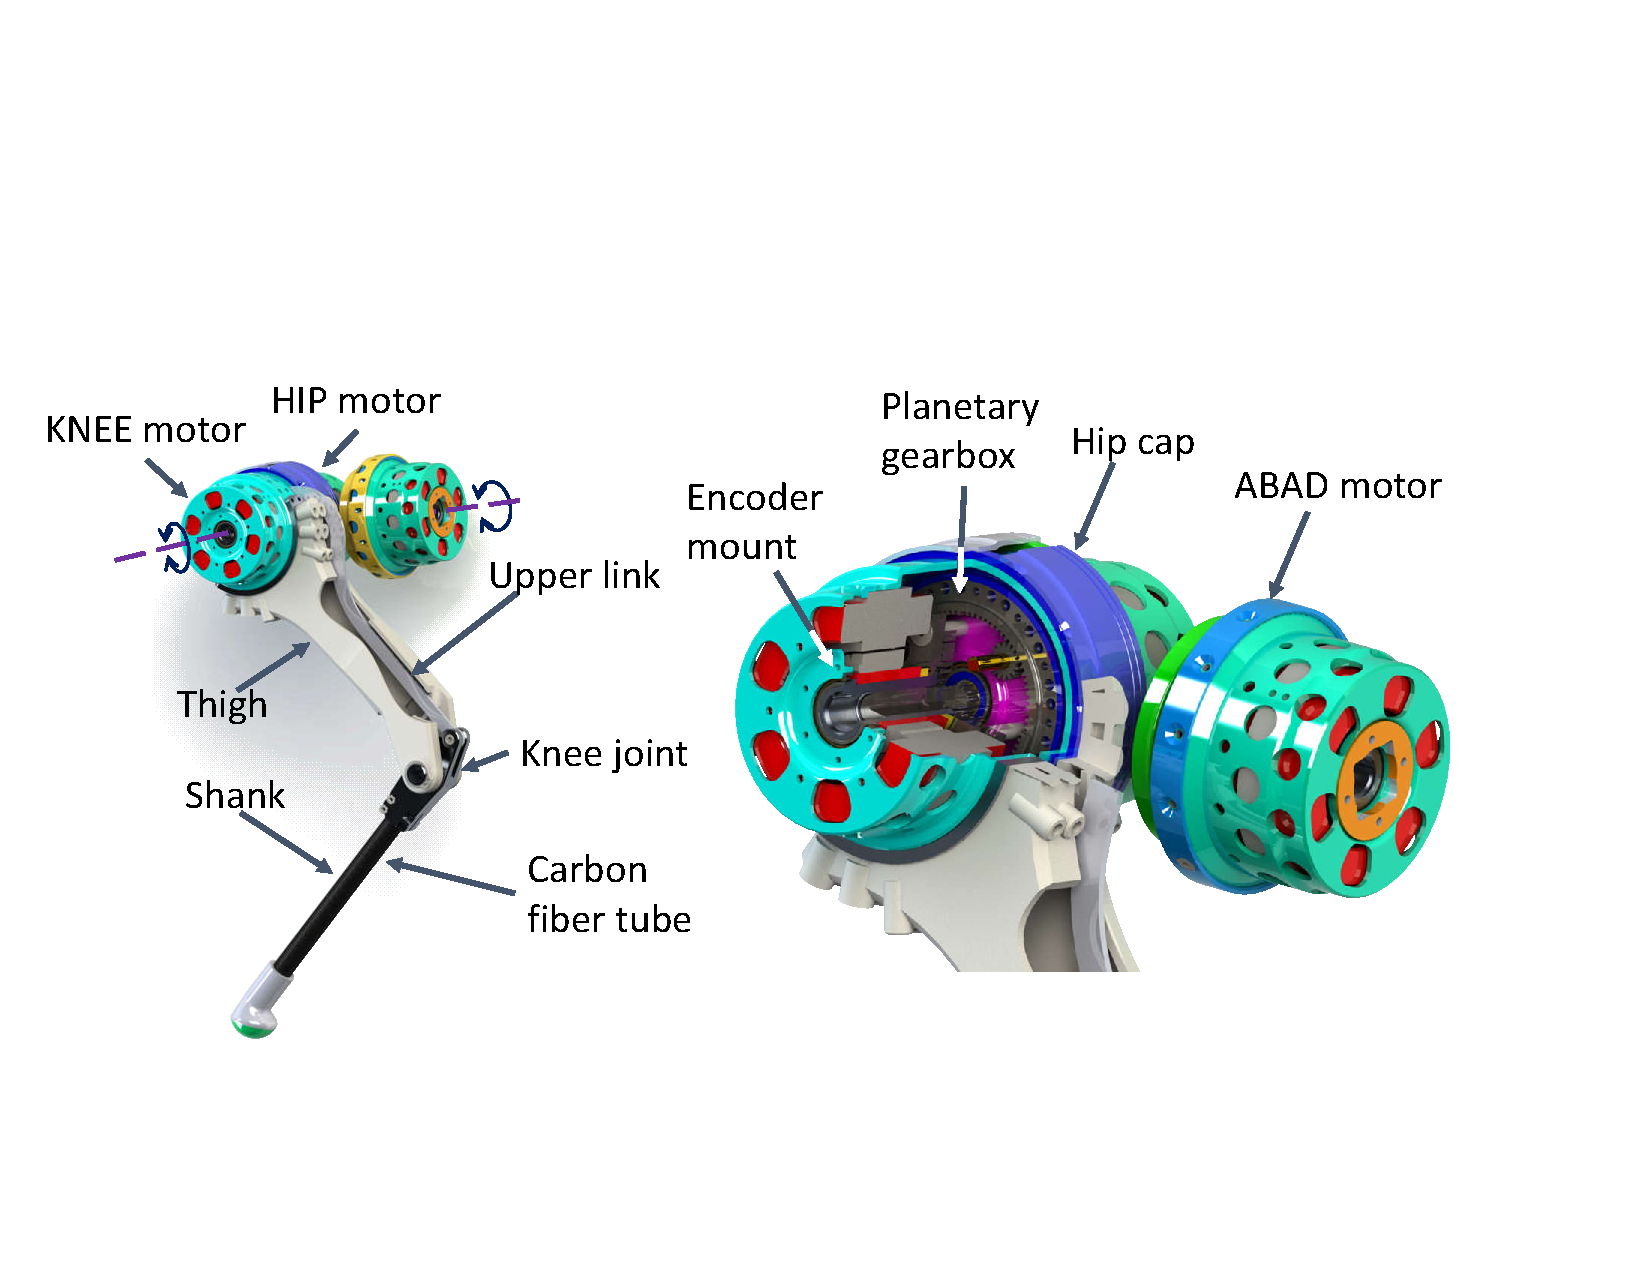
\includegraphics{SWrendering.pdf}}
	\caption{CAD Model of the Leg Module Design; (left) A side-view of the leg module with cut-out on thigh link showing the four-bar linkage design; (right) A cut-out view showing the internal structure of a motor module}
	\label{fig:LegDesign}
\end{figure}
\begin{figure}
	\centering
	\resizebox{1.0\linewidth}{!}{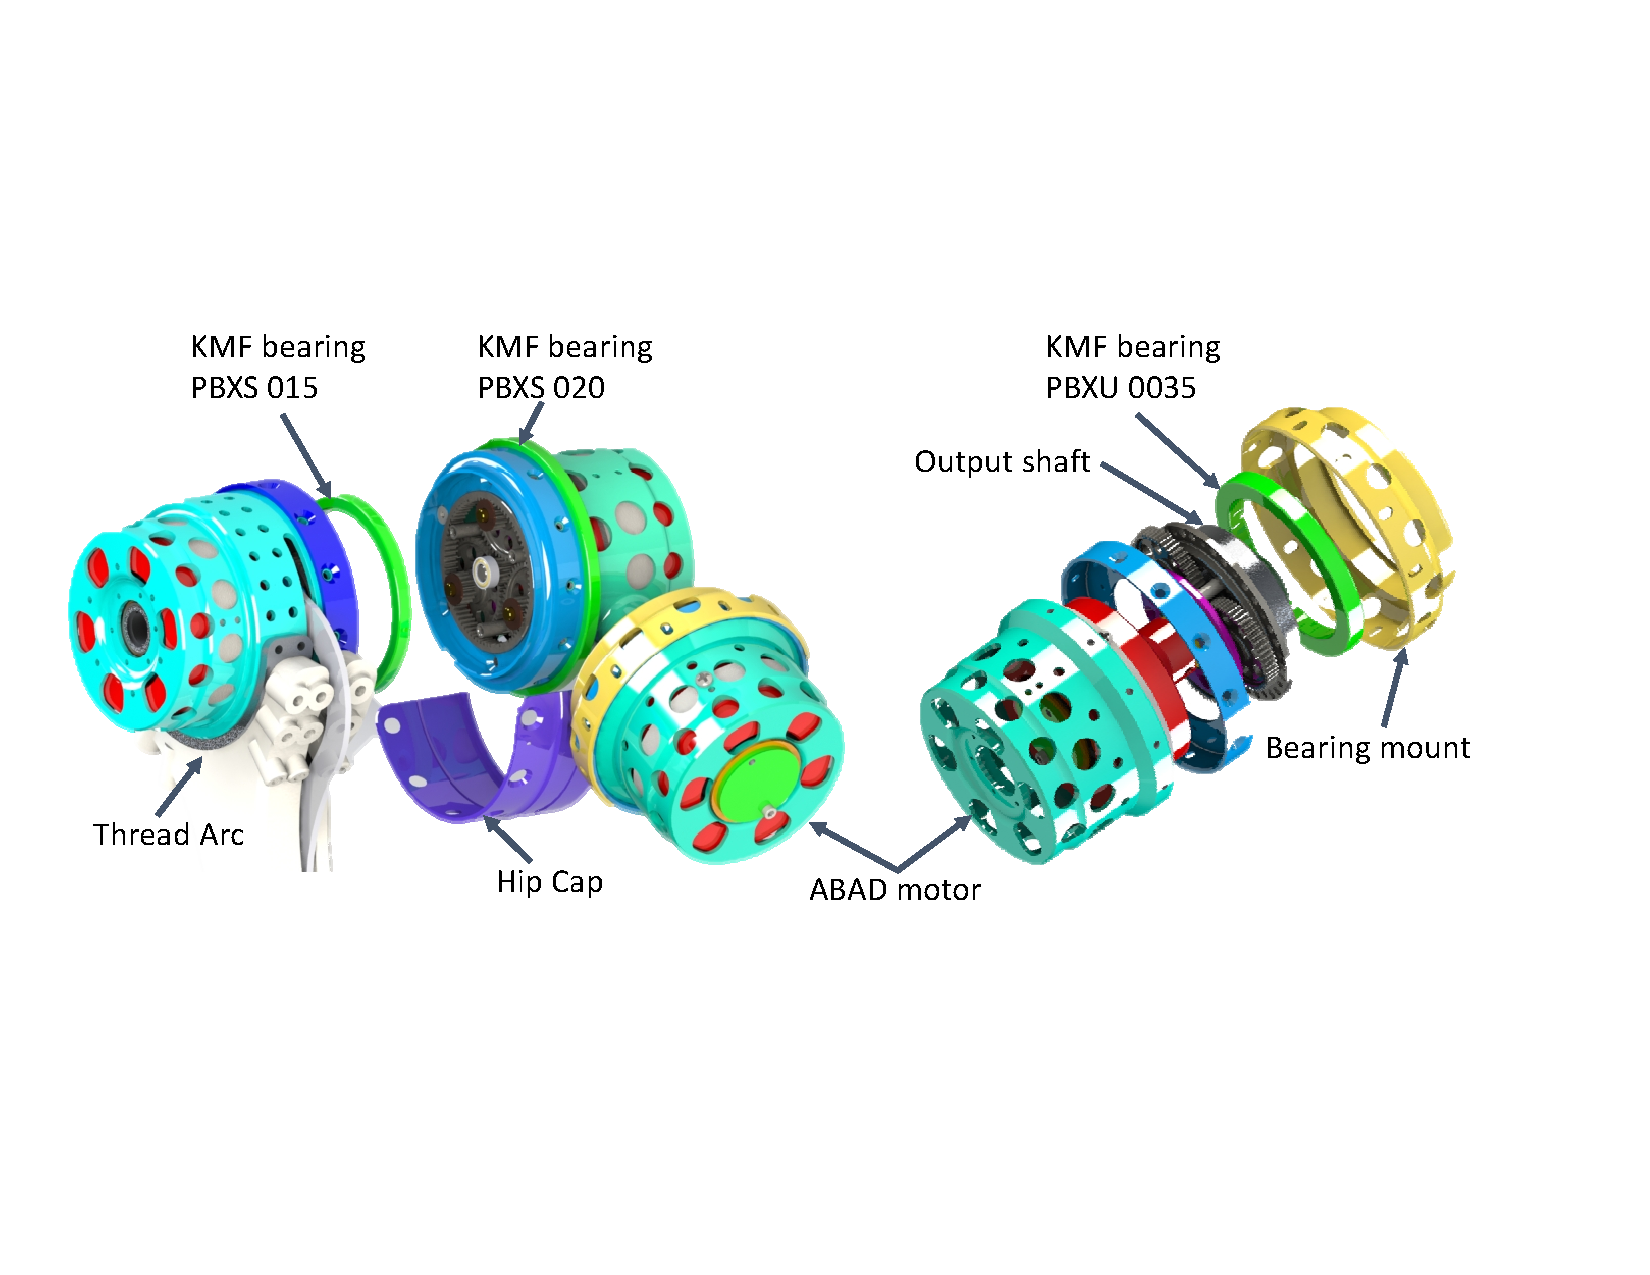
\includegraphics{KMFbearings.pdf}}
	\caption{(left) Connection Design Between HIP and KNEE Motors for Large Hip Range of Motion (ROM); (right) Exploded View of ABAD motor}
	\label{fig:KMFbearings}
\end{figure}

Each leg module is composed of three brush-less DC (BLDC) motor modules. HIP, KNEE, ABAD stand for hip joint, knee joint and abduction/adduction joints respectively. The HIP and KNEE motors are placed face-to-face and coaxially as shown in Figure \ref{fig:LegDesign}. Double supported by two thin-section bearings (KMF: PBXS020/ PBXS015), the KNEE motor could rotate $360^{\circ}$ with respect to the HIP motor. One bearing (KMF: PBXS015) is located between HIP and KNEE motors and the other one (PBXS020) is located outside of the HIP motor shell and enclosed by two hip caps. An explosive view could be found in Figure \ref{fig:KMFbearings}. The HIP motor shell's outer surface is used as one of bearing PBXS020's mating surface, and the inner surface of the Hip cap is used as the other mating surface. The hip cap is fixed to the KNEE motor and grips on the HIP motor via PBXS020 bearing, allowing the KNEE motor to rotate freely related to the HIP motor.

The ABAD motor's rotational axis is placed perpendicular to the HIP/KNEE motors' axis. The internal structure of the ABAD motor is shown in Figure \ref{fig:KMFbearings}. The torque produced by electrical coil is magnified by the planetary gearbox and transfered to the output shaft, whose motion is constrained by the bearing mount via another thin-section bearing(KMF PBXU0035). The output shaft of ABAD motor is directly connected to the HIP/KNEE module. With transmission eliminated, the workspace of the ABAD joint is not limited by the leg itself. 

\subsection{\textbf{Linkage Transmission Design}}
\label{sec:legDesign}

The linkage transmission design is shown in Figure \ref{fig:LegDesign}. The torque of the KNEE motor is transmitted to the knee joint through a four-bar linkage mechanism. Hence the KNEE motor could be put nearer to the main body and the rotary inertia could be reduced. The 3D printed hollow thigh design allows the curved upper link to travel inside without interference, while providing protection to the upper link. Consequently, the robot-human interface would be safer. In addition, the curved upper link design allows larger knee joint workspace compared with straight link design As shown in Figure \ref{fig:gearbox}, the curved link avoids the standoff (4) in the figure and gains $27^{\circ}$ more rotation angle compared with straight four-bar linkage design.

The thigh link was connected to the KNEE motor surface through four screws initially. During preliminary jumping tests it turned out that the large ground impact impulse at touch down would rip off the thread on the KNEE motor shell. To solve this problem, an additional part called thread arc was made to provide more threaded holes on the knee motor. Figure \ref{fig:KMFbearings} shows that the thread arc is attached to the KNEE motor surface and the new thigh link is fixed to the thread arc with 18 screws to evenly distribute the load.

\subsection{\textbf{Electronic System Integration}}
\label{sec:Electronics}

The electronic system of the robot leg consists of the following components: two Elmo Gold Twitter amplifiers were used for motor commutation, two RLS-RMB20 magnetic encoders were used to measure motor angle, ATI Mini40 F/T sensor was used to measure the ground reaction force created by the leg. The control loop runs at 4kHz on an Intel i5 desktop in Simulink Real-Time. 




%\include{exper}
%\include{concl}


%%%%%%%%%%%%%%%%%%%%%%%%%%%%%%%%%%%%%%%%%%%%%%%%%%%%%%%%%%%%%%%%%%%%%%%%%%%%%%%
% APPENDIX
%
\appendix
%\include{apx}

\backmatter

%%%%%%%%%%%%%%%%%%%%%%%%%%%%%%%%%%%%%%%%%%%%%%%%%%%%%%%%%%%%%%%%%%%%%%%%%%%%%%%
% BIBLIOGRAPHY
%
%\bibliographystyle{IEEE_ECE}
\bibliographystyle{IEEEtranS}
% Put references in BibTeX format in thesisrefs.bib.
\bibliography{thesisrefs}


%%%%%%%%%%%%%%%%%%%%%%%%%%%%%%%%%%%%%%%%%%%%%%%%%%%%%%%%%%%%%%%%%%%%%%%%%%%%%%%
% AUTHOR'S BIOGRAPHY
% As of 10/03/2011, Author's Biography or Vita no longer accepted by Grad College

\end{document}
\endinput
